\section{Materialwissenschaften}
\subsection{Materialklassen}

\noindent\textbf{1. Welche Eigenschaften von Materialien spielen bei der Konstruktion von Gegenständen eine Rolle?}
\indent \begin{itemize}
\item mechanische Eigenschaften
\begin{itemize}
    \item zum Beispiel $\rho$: Massendichte oder
    \item $E$: Elastizitätsmodul oder 
    \item $\sigma_y$: Streckgrenze oder
    \item $K_{1c}$: Bruchzähigkeit
\end{itemize}
    \item Thermische Eigenschaften
    \begin{itemize}
        \item  zum Beispiel maximale Temperatur für gegebene Anwendung oder
        \item $C_p$: Wärmekapazität oder
        \item $\lambda$: Wärmeleitfähigkeit oder
        \item $D \sim \frac{\lambda}{C_p}$: Diffusionskoeffizient
    \end{itemize}
    \item elektrische, optische und magnetische Eigenschaften
    \begin{itemize}
        \item zum Beispiel $\rho_e$: spezifischer elektrischer Widerstand oder
        \item $\epsilon_D$: dielektrische Konstante oder
        \item Permanentmagnet/magnetisierbar oder 
        \item $n$: Brechzahl oder
        \item $R$, $T$, $\alpha$: Reflexionskoeffizienz, Transmissionskoeffizient, Absorptionskoeffizient
    \end{itemize}
    \item chemische Eigenschaften
    \begin{itemize}
        \item zum Beispiel pH-Wert oder
        \item Wasserlöslichkeit 
    \end{itemize}
    \item sonstige Eigenschaften
    \begin{itemize}
        \item Wie gut ist Material recycelbar? 
        \item Wie teuer ist das Material?
        \item Wie gut lässt es sich verarbeiten?
    \end{itemize}
\end{itemize}

\noindent\textbf{2. Welche Materialklassen werden unterschieden?}
\indent \begin{itemize}
    \item Metalle
    \item Polymere (organische Festkörper aus langen, kohlenstoffbasierten Kettenmolekülen)
    \item Elastomere (chemisch vernetzte Polymermaterialien)
    \item Gläser (nichtkristalline (amorphe) Festkörper)
    \item Keramiken (nicht-metallische, anorganische Festkörper)
    \item Hybridmaterialien (Kombination von zwei oder mehr Materialien)
\end{itemize}
\newpage
\noindent\textbf{3. Was haben die Materialien einer Klasse gemeinsam?}
\indent \begin{itemize}
    \item ähnliche Eigenschaften
    \item ähnliche Verarbeitungsmethoden
    \item ähnliche Anwendungen
\end{itemize}

\noindent\textbf{4. Nennen Sie je drei Eigenschaften, die die Materialien jeder Materialklasse aufweisen!}
\indent \begin{itemize}
    \item Metalle
    \begin{itemize}
        \item hohe Schlagzähigkeit, Festigkeit, Verformbarkeit
        \item thermisch und elektrisch leitfähig
        \item reaktiv, leicht korrodierend
    \end{itemize}
    \item Polymere
    \begin{itemize}
        \item  niedrige Massendichte, leicht verformbar
        \item geringe Härte, niedriger Elastizitätsmodul
        \item stark druckabhängige Eigenschaften
    \end{itemize}
    \item Elastomere
    \begin{itemize}
        \item hohe Schlagzähigkeit
        \item nehmen ihre Form nach Verformung wieder an
        \item geringe Härte, niedriger Elastizitätsmodul
    \end{itemize}
    \item Gläser
    \begin{itemize}
        \item hart, aber spröde
        \item elektrische Isolatoren
        \item transparent
        \item nicht korrodierend
    \end{itemize}
    \item Kramiken
    \begin{itemize}
        \item hohe Festigkeit, Härte, Abriebfestigkeit 
        \item spröde
        \item nicht korrodierend
    \end{itemize}
\end{itemize}
\newpage
\noindent\textbf{5. Wo befinden sich die Materialien einer Klasse im $E/\rho$-Diagramm?}\\
\begin{addmargin}[25pt]{0pt}
Das $E/\rho$-Diagramm gibt Auskunft darüber welche Materialien leicht aber fest sind. Die Materialien einer Materialklasse liegen dabei ungefähr im gleichen Bereich wie Abbildung \ref{fig:E_Dichte_Diagramm} veranschaulicht.
\end{addmargin}
\begin{figure}[h]
    \centering
    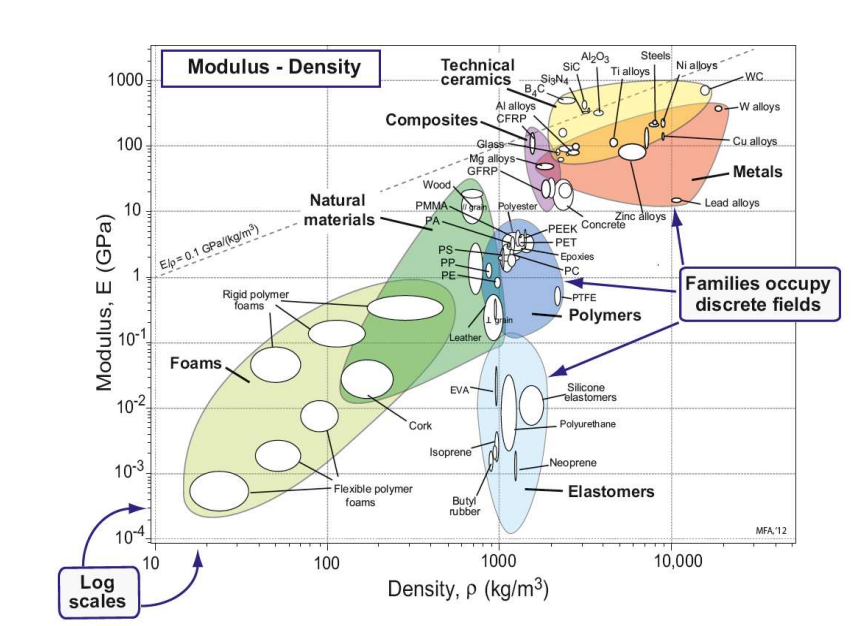
\includegraphics[width = 0.9\textwidth]{images/Materialwissenschaften/E_Dichte_Diagramm.png}
    \caption{$E/\rho$-Diagramm zur Visualisierung dass Materialklassen diskrete Bereiche einnehmen in diesem Diagramm}
    \label{fig:E_Dichte_Diagramm}
\end{figure}

\noindent\textbf{6. Aus was bestehen Nanokomposite?}\\
\begin{addmargin}[25pt]{0pt}
Bei Nanokompositen sind Füllstoffe in Nanogröße in eine Matrix eingelagert, dadurch entstehen interessante neue Eigenschaften.\\
\end{addmargin} 

\newpage
\subsection{Struktur von Festkörpern}

\noindent\textbf{1. Wie entstehen Korngrenzen?}\\
\begin{addmargin}[25pt]{0pt}
Korngrenzen entstehen wenn verschiedene Kristallkeime wachsen und größere, geordnete Kristallite bilden. Da diese Kristallite im Allgemeinen beliebig orientiert sein können wird an der Grenzfläche zwischen zwei Kristalliten die Ordnung der Einzelkristallite nicht fortgesetzt. Diese Grenze nennt man Korngrenze.
\begin{figure}[h]
    \centering
     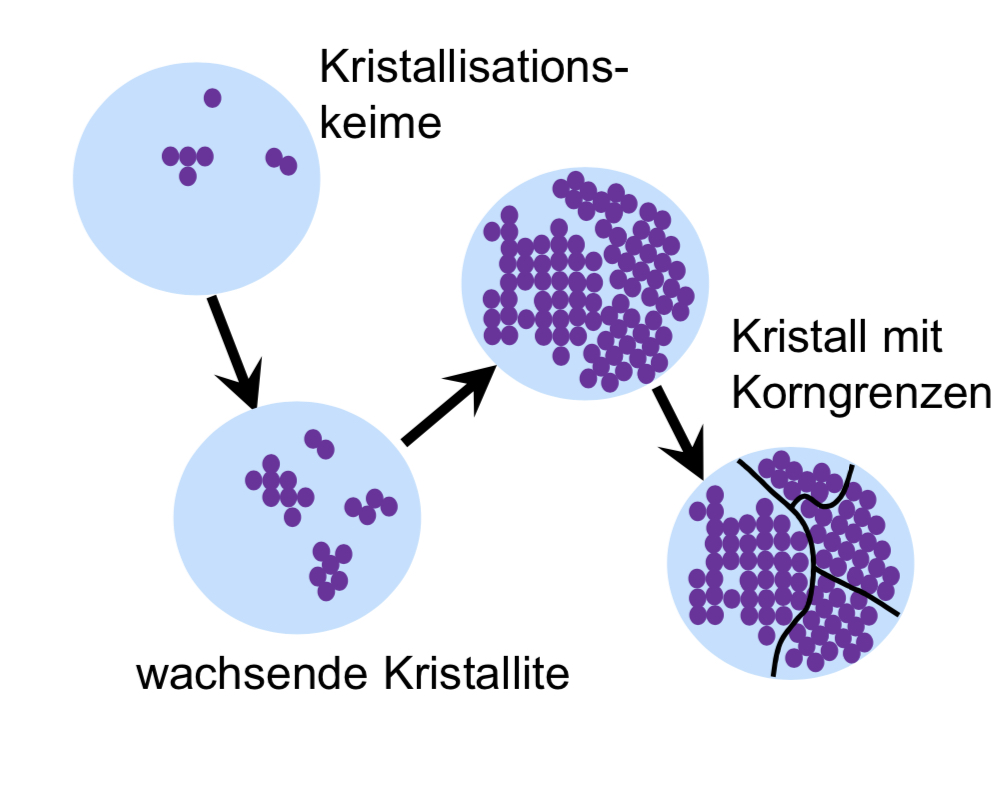
\includegraphics[width = 0.6\textwidth]{images/Materialwissenschaften/Korngrenzen.jpeg}
    \caption{Die Entstehung von Korngrenzen aufgrund des Kristallwachstums}
    \label{fig:Korngrenzen}
\end{figure}
\end{addmargin}

\noindent\textbf{2. Was sind Gläser? Aus was können sie bestehen?}\\
\begin{addmargin}[25pt]{0pt}
Gläser sind amorphe Festkörper, das bedeutet sie haben keine geordnete Gitterstruktur wie zum Beispiel die Metalle. Gläser entstehen, wenn eine Schmelze abkühlt dabei aber nicht in eine geordnete Kristallstruktur übergeht sondern die ungeordnete Struktur der flüssigen Phase erhalten bleibt. Es gibt verschiedene Arten von Gläsern, die häufigsten sind die metallischen Gläser, die vulkanischen Gläser, die organischen Gläser und die Oxidgläser. \\
\end{addmargin}

\noindent\textbf{3. Was sind Polymere und wie kristallisieren sie?}\\
\begin{addmargin}[25pt]{0pt}
Polymere sind Verbindungen aus langen Kettenmolekülen. Bei der Kristallisation von Polymeren ordnen sich in manchen Bereichen die langen Ketten parallel zueinander und auf einem Gitter an, allerdings gibt es auch Bereiche in denen diese Ordnung sich nicht ausbildet. Körper, wie Polymere, in denen sowohl kristalline als auch amorphe Bereiche auftreten nennt man \textit{teilkristallin}\\
\end{addmargin}

\noindent\textbf{4. Was sind Flüssigkristalle und welche Arten von Ordnung weisen sie auf?}\\
\begin{addmargin}[25pt]{0pt}     
In dem Zwischenbereich zwischen der kristallinen und der flüssigen Phase kann ein Körper verflüssigen aber dennoch eine gewisse Ordnung beibehalten. Dieses Zwischenstadium von Kristall und Flüssigkeit nennt man Flüssigkristall. Die verbleibende Ordnung kann in zwei Arten auftreten: in Positionsordnung, also die Moleküle haben noch einen festen Platz in der Flüssigkeit und in Orientierungsordnung, also die Moleküle haben eine vorgeschriebene Orientierung. In der Optik werden Flüssigkristalle häufig verwendet da sie doppelbrechend sind.\\
\end{addmargin}

\noindent\textbf{5. Was charakterisiert die metallische Bindung, und welche Kristallstrukturen bilden Metalle hauptsächlich aus?}\\
\begin{addmargin}[25pt]{0pt}     
Die metallische Bindung ist stark und nicht-orientiert, dadurch bilden Metalle bevorzugt Kristallgitter aus, welche hohe Packungsdichten aufweisen. Die häufigsten Strukturen sind das hcp- und das fcc-Gitter, diese haben jeweils die Koordinationszahl 12 und die Packungsdichte 0,75. In der hcp-Struktur befinden sich 6 Gitterpunkte in der konventionellen Einheitszelle, wichtige Elemente die in der hcp-Struktur kristallisieren sind Magnesium, $\alpha$-Titan und Zink. In der fcc-Struktur hingegen befinden sich 4 Gitterpunkte in der konventionellen Einheitszelle, wichtige Vertreter dieser Struktur sind Aluminium, $\gamma$-Eisen, Kupfer und Nickel. Außerdem ist die bcc-Struktur erwähnenswert, diese hat zwar nur eine Packungsdichte von 0,68 allerdings kristallisieren dennoch einige Metalle in dieser Struktur wie zum Beispiel $\alpha$-Eisen, Molybdän, $\beta$-Titan oder Chrom. \\
\end{addmargin}

\noindent\textbf{6. Was sind Zwischengitterplätze?}\\
\begin{addmargin}[25pt]{0pt}    
In einem Kristallgitter ist die Packungsdichte immer kleiner als 1, also in jedem Metallgitter ist ein kleines, freies Volumen zwischen den einzelnen Atomen, in diesen Bereich können kleinere Fremdatome eingelagert werden. Diese Poistionen zwischen den eigentlichen Gitterplätzen nennt man Zwischengitterplätze. Man unterscheidet zwischen oktahedralen und tetrahedralen Plätzen, dabei ist oktahedral der Platz in der Mitte von 6 Atomen die in einem Oktaeder angeordnet sind und analog ist tetrahedral der Platz in der Mitte von 4 Atomen an den Ecken eines Tetraeders.\\
\end{addmargin}

\noindent\textbf{7. Welche Strukturen bilden ionische Kristalle aus, und welcher Parameter spielt hierfür eine wichtige Rolle?}\\
\begin{addmargin}[25pt]{0pt}     
Ionische Kristalle bilden entweder eine einfach kubische (sc), kubisch flächenzentrierte (fcc) oder eine Zinkblendenstruktur aus. Jeder Ionenkristall versucht dabei den Abstand zwischen entgegengesetzt geladenen Ionen zu verringern, dadurch ist das Verhältnis der Ionenradien ein relevanter Faktor dafür welche Kristaallstruktur für den jeweiligen Kristall am geeignetsten ist. Im Folgenden ist $R_k$ der Radius des Kations und $R_a$ der Radius des Anions. Im Fall von $\frac{R_k}{R_a} > 0,72$ bildet sich ein sc-Kristall wie bei Caesiumchlorid (CsCl), wenn $0,33 < \frac{R_k}{R_a} < 0,72$  dann bildet sich wie bei Natriumchlorid eine fcc-Struktur und für $\frac{R_k}{R_a} < 0,33$ bildet sich eine Zinkblendenstruktur \\
\end{addmargin}

\noindent\textbf{8. Wie sind Polymere aufgebaut und was bewirkt ihre Vernetzung?}\\
\begin{addmargin}[25pt]{0pt}     
Polymere sind au langen \glqq zick-zack-förmigen\grqq Molekülen aufgebaut, dessen Hauptkette aus Kohlenstoffbindungen besteht. Diese langen Ketten können mit sich selbst vernetzen wodurch das Polymer verformbar und bei schneller Deformation elastisch wird. Verschiedene Arten der Vernetzung bewirken unterschiedliche Eigenschaften des Polymers, zum Beispiel haben Thermoplaste die Eigenschaft bei hohen Temperaturen verformbar zu sein bei niedrigen jedoch nicht.   \\
\end{addmargin}

\noindent\textbf{9. Welche Eigenschaften haben Keramiken, und welche keramischen Werkstoffe kennen Sie?}\\
\begin{addmargin}[25pt]{0pt}     
Keramiken sind sehr hart aber auch spröde. Man kann sie nicht verformen, außerdem sind sie sehr beständig gegen Chemikalien und Wärme. Ihre Leifähigkeit ist sowohl für Wärme als auch elektrischen Strom gering. Keramiken wurden bereits im 7.Jahrhundert zur Herstellung von Porzellan verwendet. Heute nutzt man Keramiken als Dielektrikum für Kondensatoren, in Verbrennungsmotoren oder als Implantate im menschlichen Körper.    \\
\end{addmargin}

\noindent\textbf{10. Was sind Silikate und welche Arten kennen Sie?}\\
\begin{addmargin}[25pt]{0pt}    
Silikate sind 4-fach negativ geladene Ionen aus einem Silizium- und vier Sauerstoffatomen. Durch die starke negative Ladung der 4 Sauerstoffatome kann diese Molekül sehr starke ionische Bindungen mit metallischen Kationen eingehen. Die beiden wichtigsten Vertreter sind Schichtsilikate und mineralische Gläser. Bei den Schichtsilikaten bilden die Silikate zweidimensionale Schichten aus, welche untereinander durch sekundäre Bindungen von den Silikaten in einem festen Abstand bleiben, dadurch kann zum Beispiel Wasser zwischen diese Schichten einlagern, damit kann man die plastischen Eigenschaften des Tons erklären. Mineralische Gläser sind dreidimensionale Silikatverbindungen, wenn in dieser 3-Struktur zusätzlich Natrium und Calcium eingelagert wird erhält man Fensterglas.   \\
\end{addmargin}









\subsection{Fehlstellen}
\noindent\textbf{1. Welche Gitterdefekte werden unterschieden?}\\
\begin{addmargin}[25pt]{0pt}     
\begin{itemize}
\item Punktdefekte ( betreffen 1-2 Atompositionen
\item Liniendefekte (eindimensional)
\item Grenzflächendefekte (zweidimensional)
\item Fremdatome\\
\end{itemize}
\end{addmargin}

\noindent\textbf{2. Welche Arten von Punktdefekten kennen Sie?}\\
\begin{addmargin}[25pt]{0pt}    
\begin{itemize}
    \item Zwischengitteratom
    \begin{itemize}
        \item Ein Atom des selben Typs kann auf einem Zwischengitterplatz sitzen
        \item Ein Fremdatom kann an einem Zwischengitterplatz sitzen
    \end{itemize}
    \item Leerstelle: Ein Gitterplatz bleibt unbesetzt
    \item Substitutionsatom: An einem Gitterplatz sitzt ein Fremdatom
\end{itemize}
\begin{figure}[h]
    \centering
    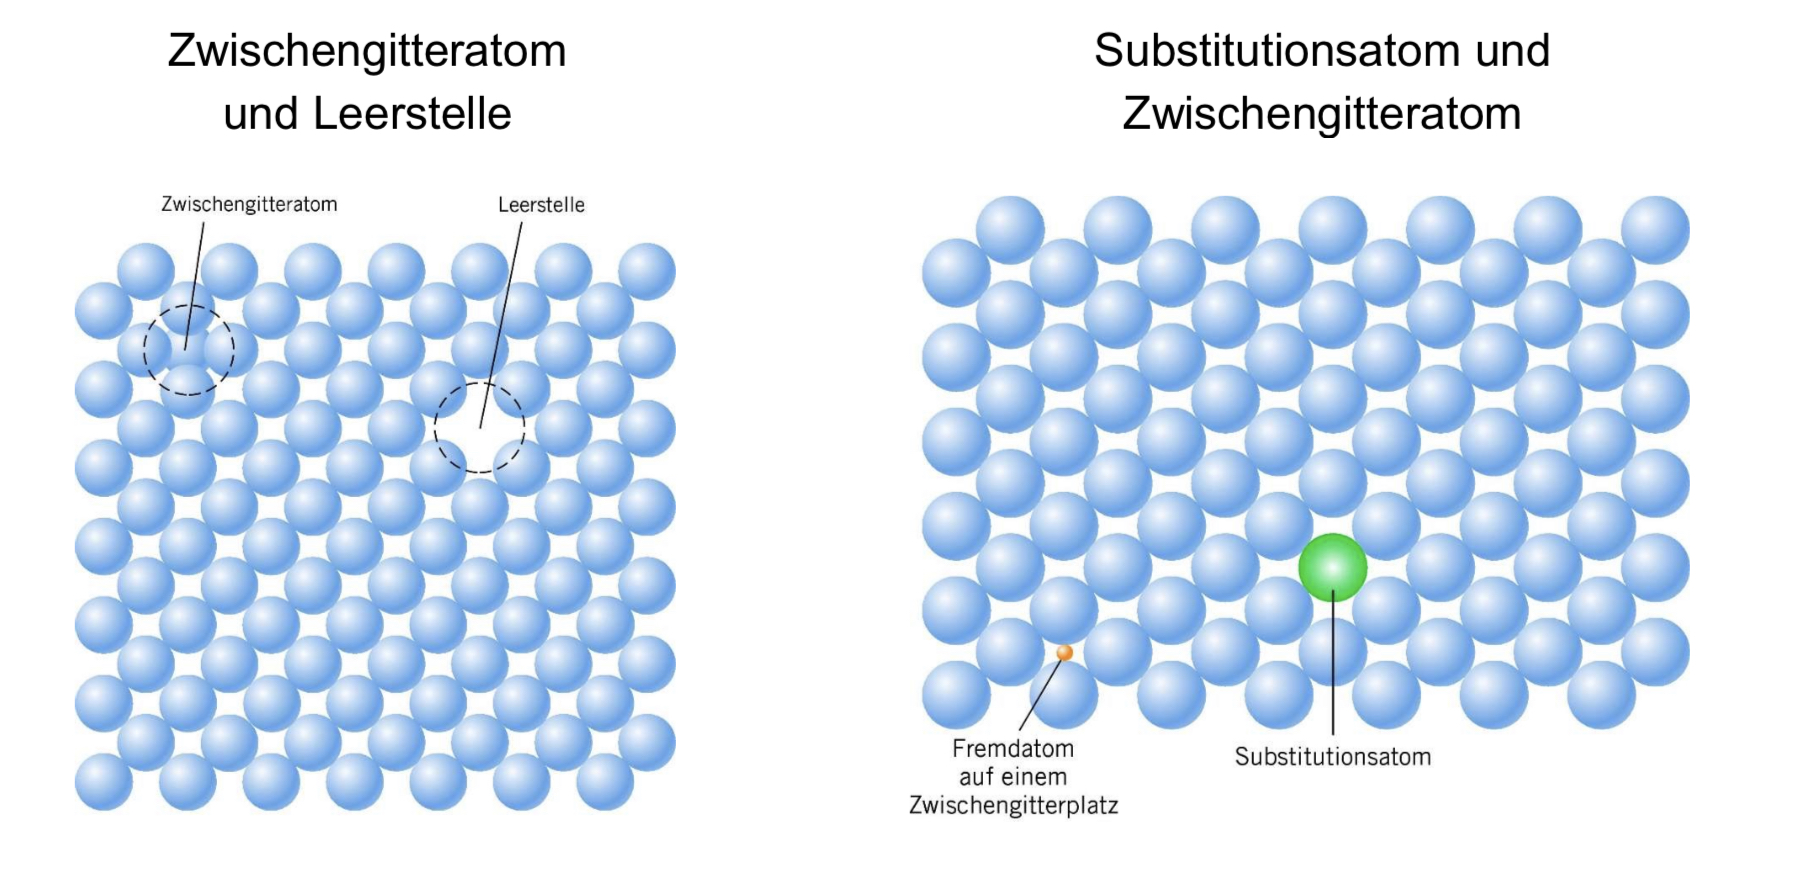
\includegraphics[width = 0.8\textwidth]{images/Materialwissenschaften/Fehlstellen.jpeg}
    \caption{Visualisierung der vier Arten von Fehlstellen}
    \label{fig:Fehlstellen}
\end{figure}
\end{addmargin}

\noindent\textbf{3. Wie können gezielt Leerstellen in ein Metall eingebracht werden?}\\
\begin{addmargin}[25pt]{0pt}    
In der flüssigen Phase einer Substanz befinden sich besonders viele Leerstellen, um diesen Zustand auch in einem Festkörper zu erreichen kann man die Flüssigkeit sehr schnell abkühlen, diesen Prozess nennt man Quenchen. Leerstellen können auch hilfreich sein da man dann gut Dotieratome in das Material einbringen kann.\\
\end{addmargin}

\noindent\textbf{4. Wie hängt die Konzentration der Leerstellen von der Temperatur ab und was ist der Grund dafür?}\\
\begin{addmargin}[25pt]{0pt}    
Die Konzentration der Leerstellen steigt stark mit der Temperatur an, besonders bei der Schmelztemperatur steigt die Anzahl der Leerstellen rasant. In der festen Phase treten Leerstellen auf da sie die Entrropie des Systems erhöhen. Die Anzahl an Leerstellen $N_V$ in der festen Phase ist: 
\begin{equation}\label{eq:Anzahl_Leerstellen}
    N_V = N\cdot e^{\frac{Q_y}{k_BT}}
\end{equation}
dabei ist $Q_y$ die Energie die zur Erzeugung einer Leerstelle nötig ist, $T$ die Temperatur und $k_B$ die Boltzmann-Konstante\\
\end{addmargin}

\noindent\textbf{5. Warum sind in Metallen Eigen-Zwischengitteratome nur in geringer Konzentration vorhanden?}\\
\begin{addmargin}[25pt]{0pt}  
In Metallen rufen Eigen-Zwischengitteratome sehr große Gitterverzerrungen hervor, dadurch ist diese Art der Fehlstelle nicht sehr wahrscheinlich. Deutlich wahrscheinlicher sind andere Defekte insbesondere die Einlagerung von Fremdatomen wie zum Beispiel Kohlenstoff in Eisen.\\
\end{addmargin}

\noindent\textbf{6. Welche Defekte werden in ionischen Kristallen unterschieden?}\\
\begin{addmargin}[25pt]{0pt}     
In ionischen Kristallen muss die gesamte Ladungsneutralität erhalten bleiben daher gibt es hier nur 2 relevante Effekte:
\begin{itemize}
    \item Schottky-Effekt
    \begin{itemize}
        \item ein Anion und ein Kation fehlen
        \item man benennt die Fehlstelle nach der Ladung die entfernt wurde nicht nach der resultierenden lokalen Restladung 
    \end{itemize}
    \item Frenkel-Effekt
    \begin{itemize}
        \item Ein Anion oder Kation verlässt seinen Gitterplatz und befindet sich nun auf einem Zwischengitterplatz
        \item dieser Prozess ist für die kleineren Ionen wahrscheinlicher
    \end{itemize}
\end{itemize}
\end{addmargin}
\newpage
\noindent\textbf{7. Welche Punktdefekte kommen in Polymeren vor?}\\
\begin{addmargin}[25pt]{0pt}   
Die langen Polymerketten können an einem Punkt im Kristall enden und dadurch dort einen Punktdefekt verursachen. Andererseits kann in den Ketten die \glqq zick-zack-Form\grqq gebrochen werden. Diesen Defekt nennt man Reneker-Defekt.
\begin{figure}[h]
    \centering
    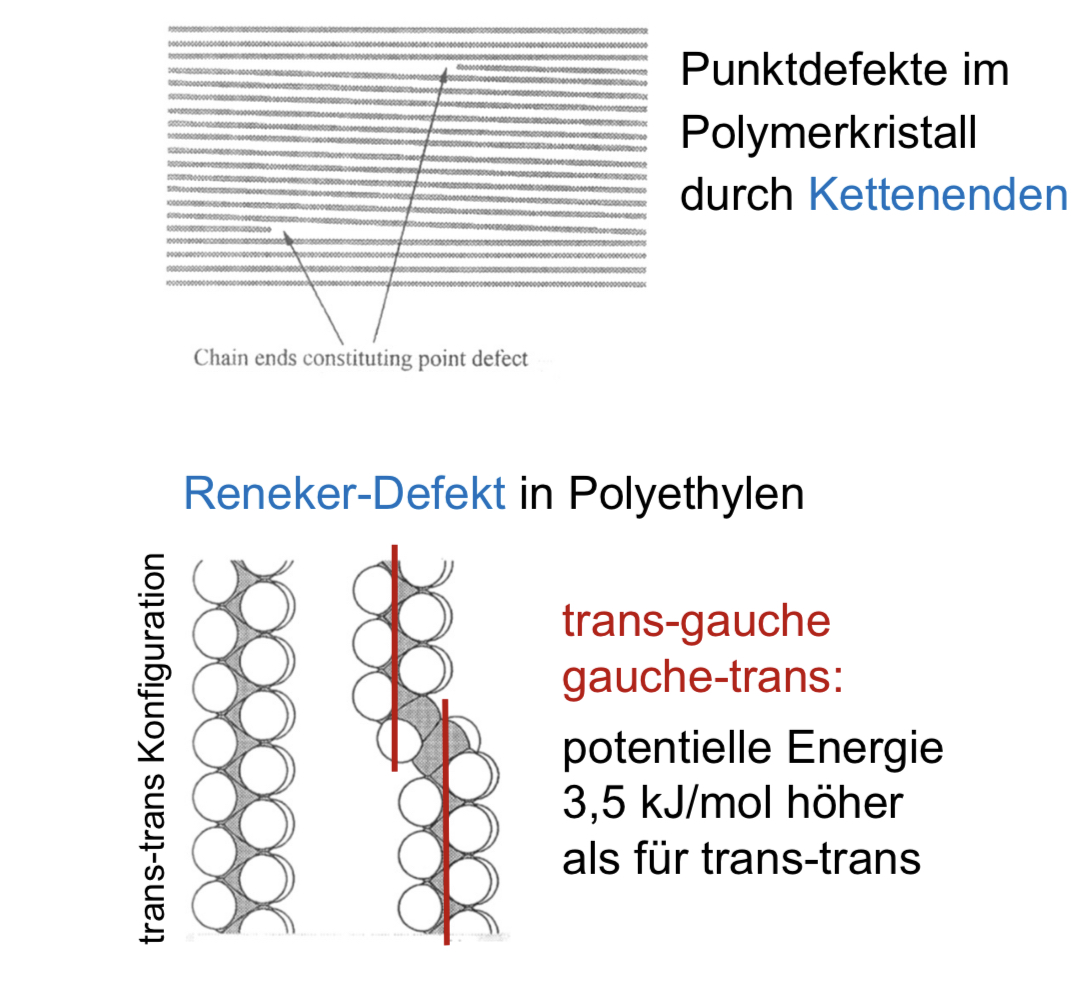
\includegraphics[width = 0.6\textwidth]{images/Materialwissenschaften/Polymerdefekte.jpeg}
    \caption{Die zwei Arten von Defekten in Polymeren. Oben sieht man das unerwartete Ende der Kette und unten ist die spontane Änderung der \glqq zick-zack-Form\grqq dargestellt}
    \label{fig:Polymerdefekte}
\end{figure}
\end{addmargin}

\noindent\textbf{8. Was sind Legierungen?}\\
\begin{addmargin}[25pt]{0pt}   
Legierungen sind das Ergebnis von gezieltem Hinzufügen von Fremdatomen in ein Metall. Dadurch kann man die Eigenschaften des Materials ändern, das wird häufig getan um die Festigkeit und Korrosionsbeständigkeit zu erhöhen.\\
\end{addmargin}

\noindent\textbf{9. Was kann passieren wenn Fremdatome zugegeben werden?}\\
\begin{addmargin}[25pt]{0pt}   
Fremdatome bewirken eine Veränderung der Eigenschaften des Materials. Bei der Zugabe von Fremdatomen kann entweder eine zweite Phase ausgebildet werden oder es entstehen Mischkristalle. Mischkristalle sind Kristalle in denen sich die Kristallstruktur des Wirtsmaterials nicht ändert und die Fremdatome gleichmäßig im Festkörper verteilt werden. Bei der Einlagerung von Fremdatomen unterscheidet man zwischen der gelösten Substanz, diese kommt in geringem Anteil vor, und dem Löser, dieser kommt in großem Anteil vor. \\
\end{addmargin}

\noindent\textbf{10. Welche Arten von Fremdatomen werden unterschieden?}\\
\begin{addmargin}[25pt]{0pt}    
Im Mischkristall gibt es 2 Arten von Fremdatomen: Substitutionsatome und Zwischengitteratome. Bei den Substitutionsatomen wird an einem Gitterpunkt ein Wirtsatom mit einem Fremdatom ausgetauscht. Bei den Zwischengitteratomen lagern sich Fremdatome auf Zwischengitterplätzen ein.\\
\end{addmargin}

\noindent\textbf{11. Unter welchen Bedingungen gibt es Substitutionsatome?}\\
\begin{addmargin}[25pt]{0pt}     
Diese Bedingungen werden in den \textit{Hume-Rothery-Regeln} festgehalten. Die erste Regel ist, dass die Atomgröße der Fremdatome nicht sehr stark von den Wirtsatomen abweichen darf. Die zweite Regel besagt, dass falls die Materialien Metalle sind sie die selbe Gitterstruktur haben müssen. Die dritte und letzte Regel schreibt vor, dass die Materialien eine ähnliche Elektronegativität haben müssen.  \\
\end{addmargin}

\noindent\textbf{12. Wo befinden sich die Fremdatome in Einlagerungsmischkristallen?}\\
\begin{addmargin}[25pt]{0pt}    
In diesem Fall sitzen die Fremdatome auf Zwischengitterplätzen. Das ist nur möglich wenn die Fremdatome einen wesentlich kleineren Radius haben als die Wirtsatome. Durch die Einlagerung auf Zwischengitterplätzen kommt es meistens zu einer Gitterverzerrung.\\
\end{addmargin}

\noindent\textbf{13. Welche Liniendefekte werden unterschieden?}\\
\begin{addmargin}[25pt]{0pt}    
Man unterscheidet bei den Liniendefekten zwischen der Stufenversetzung und der Schraubenversetzung. Die Stufenversetzung ist in Abbildung \ref{fig:Stufenversetzung} dargestellt. Bei ihr wird eine zusätzliche Halbebene in den Kristall eingefügt welche mit einer Stufe abrupt endet. Das Gitter wird aufgrund dieser zusätzlichen Ebene verzerrt. Die Schraubenversetzung, siehe Abbildung \ref{fig:Schraubenversetzung} beschreibt den Fehler, dass der obere Teil des Kristalls um einen Atomabstand verschoben ist. 

\begin{figure}[h]
  \centering
  \subfloat[Visualisierung einer Stufenversetzung\label{fig:Stufenversetzung}]{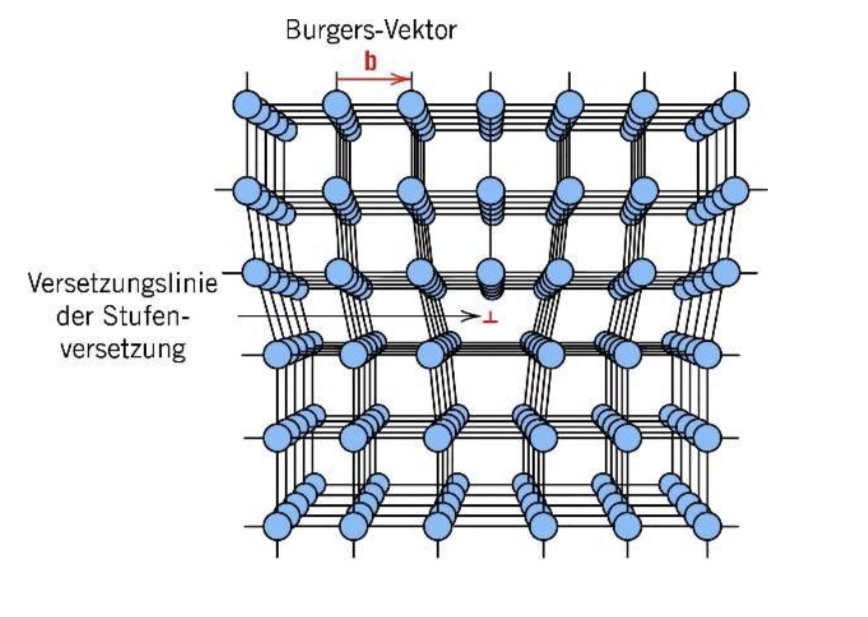
\includegraphics[height = 5cm,width=5cm]{images/Materialwissenschaften/Stufenversetzung.jpeg}}\qquad
  \subfloat[Visualisierung einer Schraubenversetzung\label{fig:Schraubenversetzung}]{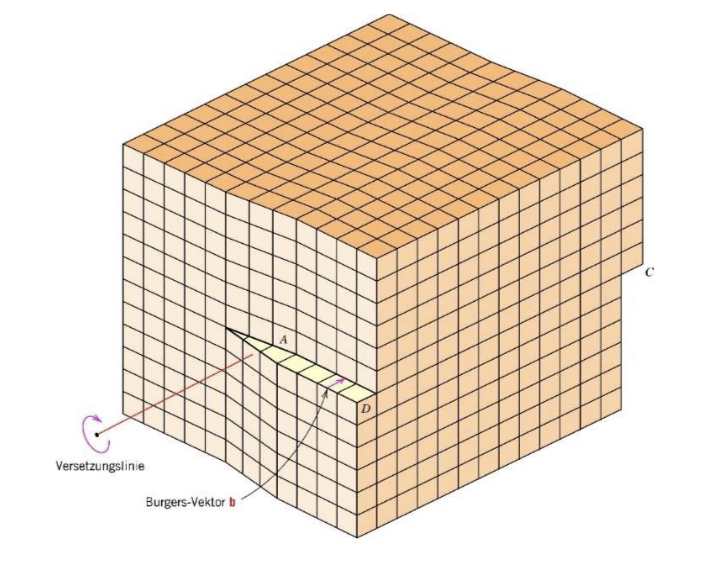
\includegraphics[height =5cm, width=5cm]{images/Materialwissenschaften/Schraubenversetzung.jpeg}}
\caption{Stufenversetzung und Schraubenversetzung}
\label{fig:Liniendefekte}
\end{figure}

\end{addmargin}

\noindent\textbf{14. Was beschreibt der Burgers-Vektor?}\\
\begin{addmargin}[25pt]{0pt}    
Der Burgers-Vektor beschreibt die Größe und Orientierung der Gitterverzerrung. Aus der Orientierung der Versetzungslinie und des Burgers-Vektors kann man die Art der Versetzung bestimmen. Falls der Burgers-Vektor senkrecht zur Versetzungslinie steht, so liegt eine Stufenversetzung vor. Liegen beide parallel so handelt es sich um eine Schraubenversetzung. \\
\end{addmargin}

\noindent\textbf{15. Welche Bewegung können die Atome bei einer plastischen Verformung durchführen?}\\
\begin{addmargin}[25pt]{0pt}   
Durch plastische Verformung können Stufenversetzungen verschoben werden, der Defekt bewegt sich dabei ähnlich wie eine Raupe fort. Dieser Prozess geht so lange bis der Defekt am Rand des Materials ist. Das ist der Grund warum man Metalle nachdem sie einmal verformt sind nur sehr schwer wieder in den Ursprungszustand zurückbringen kann. \\
\end{addmargin}

\noindent\textbf{16. Was sind Flächenversetzungen?}\\
\begin{addmargin}[25pt]{0pt}    
Flächenversetzungen sind Grenzflächen, welche Materialbereiche mit unterschiedlicher Kristallstruktur voneinander abgrenzen. Das können zum Beispiel Korngrenzen, Phasengrenzen oder die Oberfläche des Körpers sein. Weiterhin sind die Zwillingsgrenzen und der Stapelfehler Vertreter der Flächenversetzungen.  \\
\end{addmargin}

\noindent\textbf{17. Was ist an Kristalloberflächen anders als im Volumen?}\\
\begin{addmargin}[25pt]{0pt}   
Die Atome an den Oberflächen haben weniger Nachbarn also eine geringere Koordinationszahl. Dadurch haben die Atome an der Oberfläche eine höhere Energie als die im Volumen des Materials. Das System strebt die Minimierung dieser Energie an, also eine möglichst kleine Oberfläche, dadurch sind kugelförmige Tropfen oder Nanopartikel energetisch bevorzugt.\\
\end{addmargin}

\noindent\textbf{18. Welche Korngrenzen kennen Sie?}\\
\begin{addmargin}[25pt]{0pt}    
Die nur wenige Atomschichten dicken Übergänge zwischen zwei Bereichen mit unterschiedlicher Kristallausrichtung werden als Korngrenzen bezeichnet. Falls der unterschied in der Ausrichtung der angrenzenden Körner nur sehr klein ist spricht man von Kleinwinkel-Korngrenzen, diese kann man näherungsweise durch mehrere Stufenversetzungen beschreiben. Ist diese Näherung nicht möglich spricht man von der Großwinkel-Korngrenze. \\
\end{addmargin}

\noindent\textbf{19. Was sind Zwillingsgrenzen?}\\
\begin{addmargin}[25pt]{0pt}    
Zwillingsgrenzen sind Korngrenzen die als Spiegelachse für die Kristallstruktur fungieren. Ein Beispiel für diese Zwillingsgrenze kann man in Abbildung \ref{fig:Zwillingsgrenze} sehen. Zwillingsgrenzen entstehen zum Beispiel durch Scherung. 
\begin{figure}[h]
    \centering
    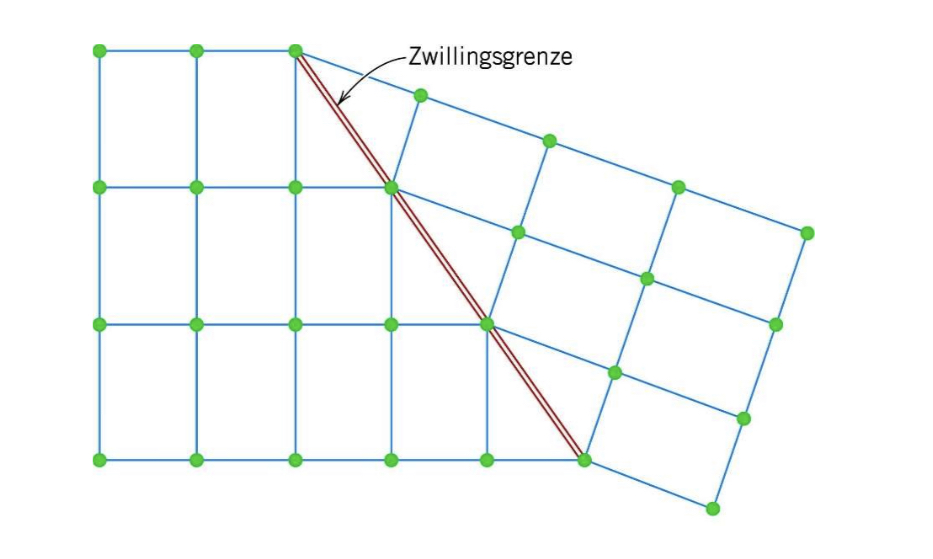
\includegraphics[width = 0.6\textwidth]{images/Materialwissenschaften/Zwillingsgrenze.jpeg}
    \caption{Visualisierung von einer Zwillingsgrenze}
    \label{fig:Zwillingsgrenze}
\end{figure}\\
\end{addmargin}



\subsection{Diffusion}
\noindent\textbf{1. Was ist Diffusion?}\\
\begin{addmargin}[25pt]{0pt}
Diffusion ist der Massetransport aufgrund der regellosen Bewegung von Atomen. In unserem Fall betrachten wir Festkörper und dabei ist die Diffusion die Bewegung de Atome durch das Kristallgitter.\\
\end{addmargin} 


\noindent\textbf{2. Welche Arten der Diffusion werden unterschieden?}\\
\begin{addmargin}[25pt]{0pt}
Im Wesentlichen werden 2 Arten der Diffusion unterschieden. Die erste Variante ist die Leerstellendiffusion, bei dieser springt ein Atom von seinem Gitterplatz zu einem benachbarten leeren Gitterplatz. Das geschieht zum Beispiel in Metallen bei hohen Temperaturen. Die zweite Möglichkeit ist die interstitielle Diffusion, bei dieser bewegt sich ein Zwischengitteratom von einem Zwischengitterplatz zum Nächsten.  Dieser Mechanismus geschieht bei Metallen mit kleinen Fremdatomen wie Wasserstoff, Kohlenstoff, Sauerstoff oder Stickstoff.\\
\end{addmargin} 

\noindent\textbf{3. Warum ist die interstitielle Diffusion schneller als die Leerstellendiffusion?}\\
\begin{addmargin}[25pt]{0pt}
Das liegt daran, dass die Zwischengitteratome kleiner und beweglicher sind sind als die Wirtsatome. Außerdem gibt es mehr unbesetzte PLätze wodurch die Bewegung wahrscheinlicher wird. Ein dritter Punkt von Relevanz bei der Diffusionsgeschwindigkeit sind die schwächeren Bindungen an den ZWischengitteratomen im Vergleich zu Atomen im Gitter. \\
\end{addmargin} 

\noindent\textbf{4. Wie hängt die Diffusionsstromdichte von den Konzentrationsgradienten ab?}\\
\begin{addmargin}[25pt]{0pt}
Die Diffusionsstromdichte ist proportional zum Konzentrationsgradienten. 
\begin{equation}\label{eq:Fick1}
    \mathbf{J}(x,y,z) = -D\cdot \nabla c(x,y,z) 
\end{equation}
Die Proportionalitätskonstante ist der Diffusionskoeffizient $D$ mit der Einheit $\left[ \frac{\si{m}^2}{\si{s}}\right]$. Der Diffusionskoeffizient ist eine Stoffeigenschaft die von den beiden beteiligten Stoffen abhängt. Den Zusammenhang in Gleichung \ref{eq:Fick1} nennt man \textit{1. Fick'sches Gesetz}. Das Minuszeichen in dieser Gleichung besagt, dass der Diffusionsstrom von Orten hoher Konzentration zu Orten niedriger Konzentration geht.\\
\end{addmargin} 

\noindent\textbf{5. Wie lautet das zweite Fick'sche Gesetz und was beschreibt es?}\\
\begin{addmargin}[25pt]{0pt}
Das zweite Fick'sche Gesetz lautet in einer Dimension:
\begin{equation}\label{eq:Fick2}
    \frac{\partial c}{\partial t} + \frac{\partial J}{\partial x} = 0
\end{equation}
In 3 Dimensionen wird die örtlichen Ableitung in Gleichung \ref{eq:Fick2} mit dem Gradienten ersetzt. Das zweite Fick'sche Gesetz besagt, dass die Differenz der Teilchenströme die in ein Volumen hinen- bzw. hinausfließen der Änderung der Konzentration im Volumen entspricht.\\
Man kann \ref{eq:Fick2} und Gleichung \ref{eq:Fick1} kombinieren un derhält eine Alternative Formulierung für das zweite Fick'sche Gesetz:
\begin{equation}\label{eq:Fick2_Alternative}
    \frac{\partial c}{\partial t} = D \Delta c
\end{equation}
Dabei ist $\Delta$ der Laplace-Operator der die zweiten örtlichen Ableitungen erhält. Das zweite Fick'sche Gesetz ist also eine partielle Differentialgleichung für die Stoffmengenkonzentration.\\
\end{addmargin} 

\noindent\textbf{6. Wie sieht das Konzentrationsprofil an einer Grenzfläche aus?}\\
\begin{addmargin}[25pt]{0pt}
An einer Grenzfläche (wie in Abbildung \ref{fig:grenzflächendiffusion} für Kupfer und Nickel zu sehen) sind die Konzentrationen zum Zeitpunkt $t = 0$ scharfe Stufenfunktionen mit der Unstetigkeitsstelle am Ort der Grenzfläche. Mit der Zeit werden allerdings immer mehr Atome von beiden Substanzen über die Grenzfläche diffundieren und so wird sich die Konzentration auch verändern. Die neue Funktion des Konzentrationsprofils ist eine von Ort und Zeit abhängige Gauß'sche Fehlerfunktion. \\

\begin{figure}[h]
    \centering
    \includegraphics[width = 0.9\textwidth]{images/Materialwissenschaften/Grenzflächendiffsuion.jpeg}
    \caption{Diffusion an einer Cu-Ni-Grenzfläche zum Zeitpunkt 0 und zu einem späteren Zeitpunkt }
    \label{fig:grenzflächendiffusion}
\end{figure}
\end{addmargin} 

\noindent\textbf{7. Wie hängen Diffusionskoeffizienten von der Temperatur ab und was sagt das über den Prozess?}\\
\begin{addmargin}[25pt]{0pt}
Der Funktionalzusammenhang für den Diffusionskoeffizienten von der Temperatur lautet:
\begin{equation}\label{eq:Diffisuion_von_Temperatur}
    D(T) = D_0\cdot e^{-\frac{Q_d}{RT}}
\end{equation}
Dabei ist $D_0$ ein temperaturunabhängiger Vorfaktor, $Q_d$ die Aktivierungsenergie in $\frac{\si{J}}{\si{mol}}$ und $R$ die universelle Gaskonstante.\\
\end{addmargin} 

\noindent\textbf{8. Was ist ein Arrhenius-Diagramm und was kann man darin ablesen? }\\
\begin{addmargin}[25pt]{0pt}
Im Arrhenius-Diagramm (Abbildung \ref{fig:arrhenius}) wird der Diffusionskoeffizient logarithmisch gegen den Kehrwert der Temperatur aufgetragen. Daraus kann man dann die Aktivierungsenergie und den Faktor $D_0$ ablesen. Der Schnittpunkt mit der $D$-Achse ist dabei der Vorfaktor $D_0$ und die Aktivierungsenergie bestimmt man aus der Steigung der entstehenden Geraden $-\frac{Q_d}{R\cdot\ln{10}}$ der Faktor $\ln{10}$ kommt daher, dass man den dekadischen Logarithmus zum plotten verwendet.\\
\begin{figure}[h]
    \centering
    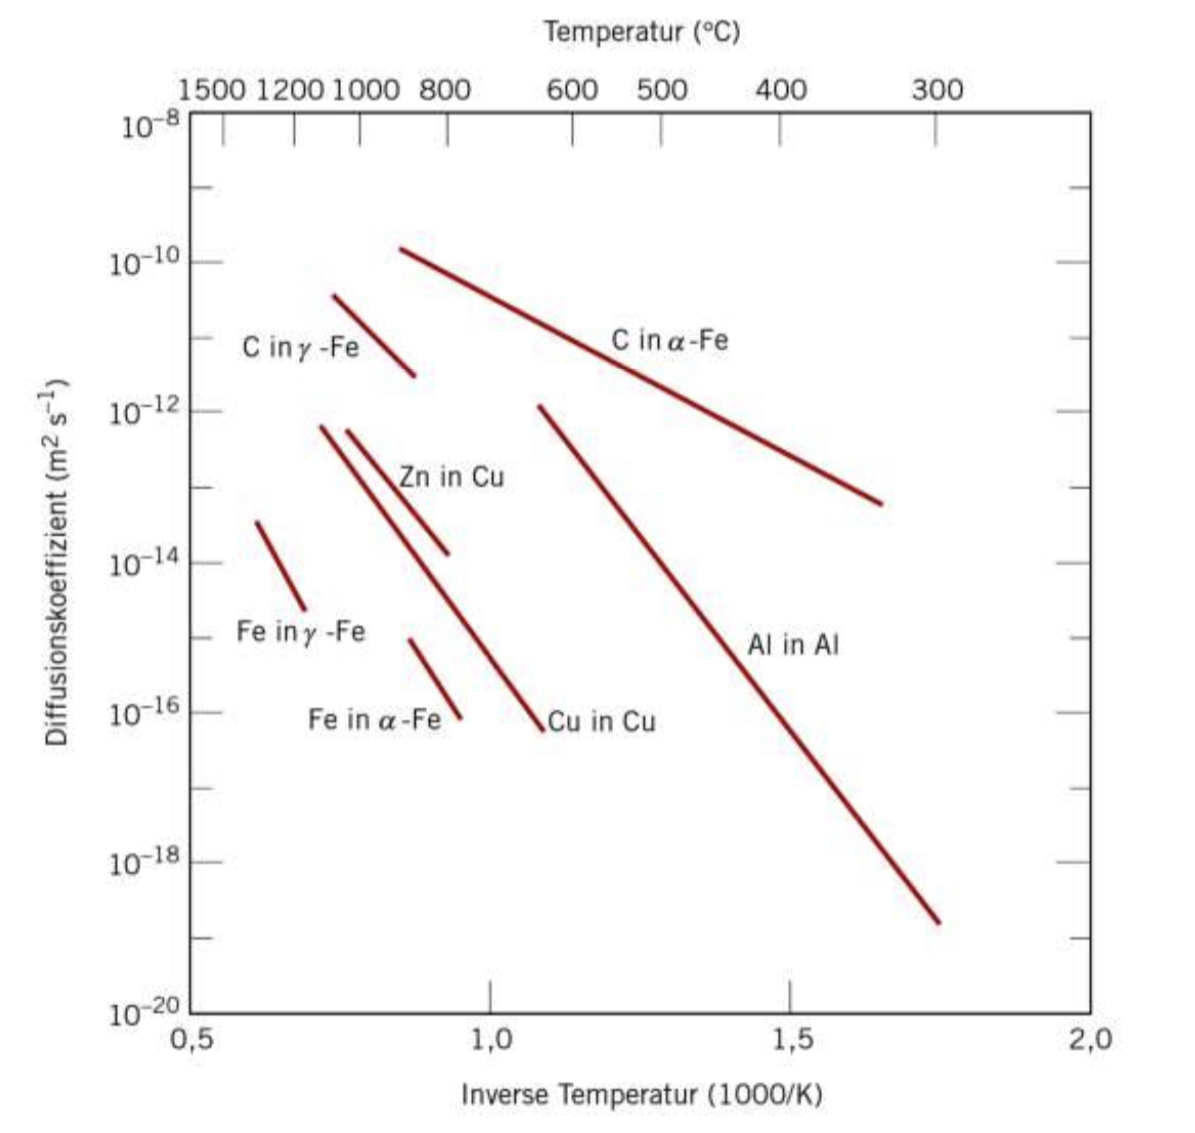
\includegraphics[width = 0.8\textwidth]{images/Materialwissenschaften/Arrhenius.jpeg}
    \caption{Arrhenius-Diagramm für verschiedene Stoffe}
    \label{fig:arrhenius}
\end{figure}
\end{addmargin} 

\noindent\textbf{9. Wie hängt der Diffusionskoeffizient von der Sprungweite und Sprungfrequenz ab?}\\
\begin{addmargin}[25pt]{0pt}
Aus der atomistischen Betrachtung des Diffusionskoeffizienten kann man diesen abhängig von der Weite eines Sprunges $\lambda$ und der Sprungfrequenz $\Gamma$, also der Häufigkeit der Sprünge, ausdrücken. Dieser Zusammenhang lautet:
\begin{equation}\label{eq:Diffusion_atomistisch}
    D = \frac{\lambda^2}{6}\Gamma
\end{equation}\\
\end{addmargin} 

\noindent\textbf{10. Warum ist die Diffusion ein aktivierter Prozess? }\\
\begin{addmargin}[25pt]{0pt}
Diffusion kann nicht bei beliebig kleinen Energien stattfinden, da die diffundierenden Atome eine gewisse Energie benötigen um im Gitter einen Platz weiter springen zu können. Das bedeutet das Diffusion erst ab der Aktivierungsenergie $Q_d$  möglich ist. Prozess die erst ab einer gewissen Grenze starten nennt man aktivierte Prozesse.\\
\end{addmargin} 

\newpage
\subsection{Elastisches Verhalten}
\noindent\textbf{1. Welche Experimente werden durchgeführt um den Elastizitätsmodul und den Schubmodul zu messen?}\\
\begin{addmargin}[25pt]{0pt}
\begin{itemize}
    \item Zugversuch
    \begin{itemize}
        \item uniaxiale Dehnung entlang der Achse eines elastischen Stabs
        \item Stab wird länger entlang Kraftwirkung und schmaler senkrecht zur Kraft
        \item Dehnung entlang der Kraft ist definiert als $\epsilon = \frac{\Delta l}{l_0}$
        \item $\Delta l :=$ Längenänderung bei angelegter Kraft; $l_0 :=$ ursprüngliche Länge des Stabs
        \item Spannung $\sigma$ ergibt sich aus Elastizitätsmodul $E$ und Dehnung $\epsilon$: $\sigma = E\cdot\epsilon$ 
        \item Spannung ist ebenfalls über angelegte Kraft $F$ und ursprüngliche Querschnittsfläche $A_0$ definiert: $\sigma = \frac{F}{A_0}$
    \end{itemize}
    \item Druckversuch
    \begin{itemize}
        \item wie Zugversuch aber Stauchung anstatt Dehnung 
        \item Unterschied: Kraft hat anderes Vorzeichen
    \end{itemize}
    \item Scherversuch
    \begin{itemize}
        \item Kraft wirkt nicht mehr senkrecht auf Oberfläche sondern parallel
        \item Scherspannung $\tau$ ist analog zu Spannung beim Zugversuch definiert: $\tau = \frac{F}{A_0}$
        \item Scherdehnung $\gamma$ ist der Tangens des Winkels $\theta$ um den sich Probe verdreht: $\gamma = \tan\theta$
        \item Es gilt wieder: $\tau = G\cdot\gamma$, dabei ist $G$ der Schubmodul
    \end{itemize}
    \item Torsionsversuch
    \begin{itemize}
        \item analog zu Scherversuch aber die betrachtete Verdrehung ist anders
        \item es wird Torsionsmoment angelegt wodurch der Körper um seine eigene Achse eingedreht wird
    \end{itemize}
\end{itemize}
Alle Versuche sind nochmal in Abbildung \ref{fig:Modulnversuche} visualisiert

\begin{figure}[h]
    \centering
    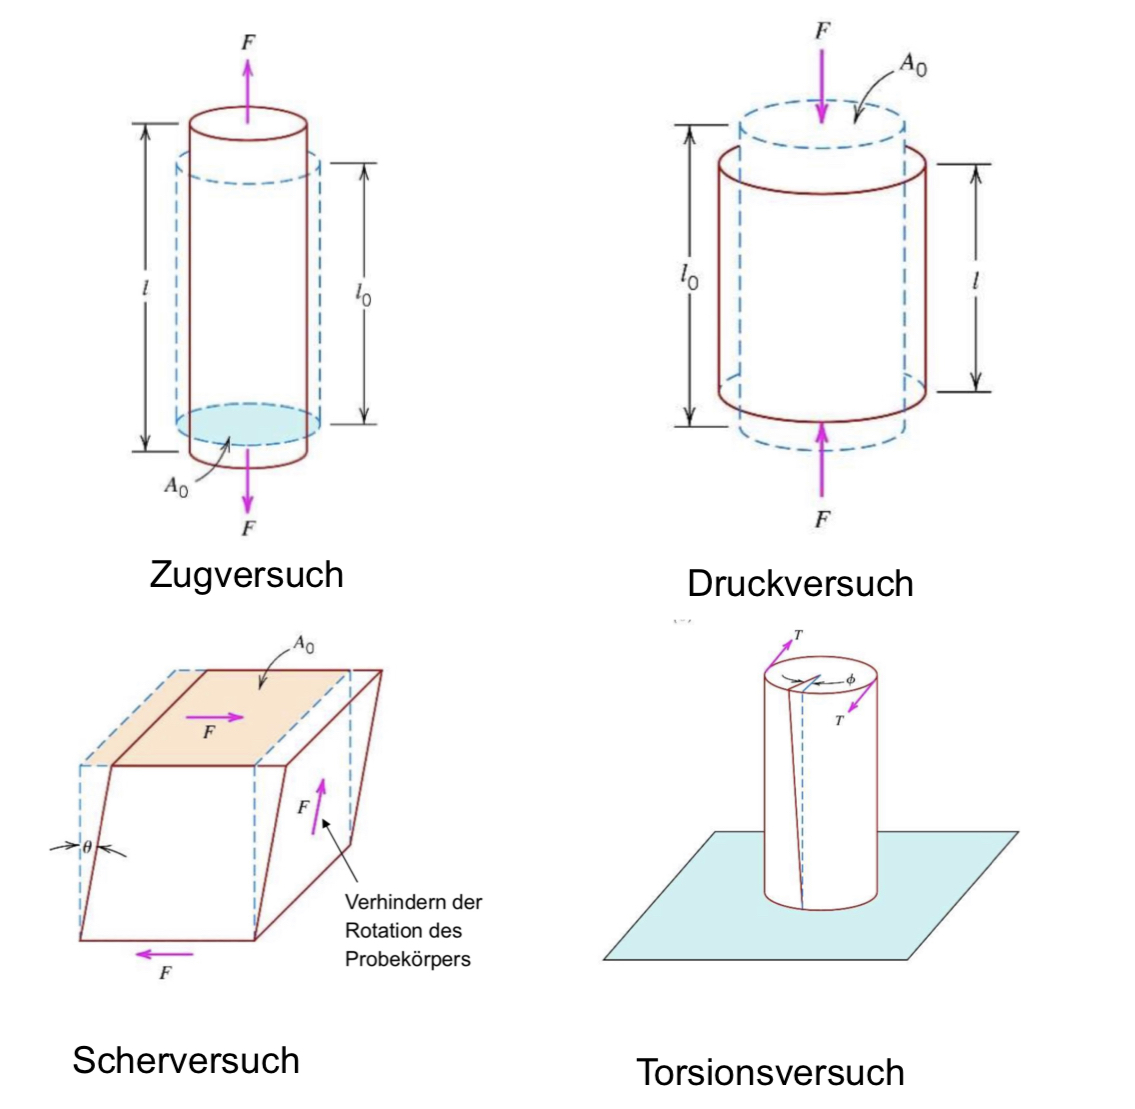
\includegraphics[width = 0.8\textwidth]{images/Materialwissenschaften/Modulnversuche.jpeg}
    \caption{Die 4 verschiedenen Versuche zur Bestimmung des Elastizitätsmoduls und des Schubmoduls visualisiert}
    \label{fig:Modulnversuche}
\end{figure}
\end{addmargin} 


\noindent\textbf{2. Was besagt das Hooke'sche Gesetz und unter welchen Bedingungen gilt es bei Metallen?}\\
\begin{addmargin}[25pt]{0pt}
Das Hooke'sche Gesetz sagt einen linearen Zusammenhang zwischen Dehnung $\epsilon$ und Dehnung $\sigma$ voraus. Das gilt für Metalle allerdings nur in einem gewissen Bereich da bei zu großen Belastungen plastische Verformungen auftreten. Die Proportionalitätakonstante zwischen den beiden Größen ist der Elastizitätsmodul. Im Bereich des Hooke'schen Gesetzes sind die Deformationen reversibel. Das Hooke'sche Gesetz lautet:
\begin{equation}\label{eq:Hooke_Gesetz}
    \sigma = E \cdot \epsilon
\end{equation}
\end{addmargin} 


\noindent\textbf{3. Was passiert beim Zugversuch in Querrichtung und wie ist die Poisson-Zahl definiert?}\\
\begin{addmargin}[25pt]{0pt}
Beim Zugversuch mit angelegter Kraft in z-Richtung wird der Körper in x- und y-Richtung seinen Querschnitt verringern. Dabei wird angenommen, dass die Dehnungen in Querrichtung gilt: $\epsilon_x = \epsilon_y$. Die Poisson-Zahl ist das Verhältnis der Querdehnung zur Längsdehnung:
\begin{equation}\label{eq:Definition_Poisson_Zahl}
\nu = -\frac{\epsilon_x}{\epsilon_z}
\end{equation}
Das negative Vorzeichen kommt daher, dass die Querdehnung kleiner als null ist. Unter der Annahme, dass sich das Volumen des Körpers beim Zugversuch nicht ändert müsste für die Poisson-Zahl $\nu = \frac{1}{2}$ gelten. Allerdings zeigen Experimente, dass diese Annahme nicht berechtigt ist und die Poisson-Zahl für isotrope Materialien ungefähr $\frac{1}{4}$ ist.\\ 
\end{addmargin} 


\noindent\textbf{4. Welcher Zusammenhang besteht zwischen dem Elastizitätsmodul und dem Schubmodul?}\\
\begin{addmargin}[25pt]{0pt}
Der Elastizitätsmodul $E$ und der Schubmodul $G$ sind über die Poisson-Zahl $\nu$ miteinander verknüpft. Ihr Zusammenhang lautet:
\begin{equation}\label{eq:zusammenhang_E_G_nu}
    E = 2G(1+\nu)
\end{equation}
Für viele Metalle ist dabei $G \approx 0,4 E$ weil $\nu \approx \frac{1}{4}$\\
\end{addmargin} 


\noindent\textbf{5. Aus welchen Beiträgen setzt sich beim Zugversuch die vom System geleistete Arbeit zusammen?}\\
\begin{addmargin}[25pt]{0pt}
Streckt man einen Körper um eine Länge $\si{d}l$ so muss man Arbeit verrichten um der Rückstellkraft $F_r$ des elastischen Zusammenziehens entgegenzuwirken. Eine zweite Komponente der geleisteten Arbeit tritt auf, da man beim Dehnen das Volumen des Körpers ändert und so Volumenänderungsarbeit $p\si{d}V$ verrichten muss, die gesamte aufzubringende Arbeit $\si{d}W$ ist dann:
\begin{equation}\label{eq:geleistete_Arbeit_Zugversuch}
    \delta W = -F_r \si{d}l + p\si{d}V
\end{equation}
Da man von reversiblem Dehnen ausgeht kann man auch noch die transportierte Wärme $\delta Q = T\si{d}S$ bestimmen und so mit dem ersten Hauptsatz der Thermodynamik die Änderung der inneren Energie $\si{d}U$ des Systems:
\begin{equation}\label{eq:innere_Energie_Zugversuch}
    \si{d}U = \delta Q - \delta W = T\si{d}S + F_r \si{d}l - p\si{d}V
\end{equation}
\end{addmargin} 


\noindent\textbf{6. Aus welchen Beträgen setzt sich die elastische Rückstellkraft zusammen?}\\
\begin{addmargin}[25pt]{0pt}
Die elastische Rückstellkraft hat eine enthalpische Komponente $F_{r,i}$ und eine entropische Komponente $F_{r,e}$. Diese unterschiedlichen Komponenten entstehen dadurch, dass zugeführte mechanische Arbeit entweder als innere Energie, also als Veränderung der atomaren Abstände oder der Bindungswinkel, gespeichert werden kann oder in Form von Wärme an die Umgebung abgegeben wird wodurch sich die Ordnung im Probenkörper erhöht.\\
\end{addmargin} 


\noindent\textbf{7. Welcher Beitrag dominiert bei Metallen? Worauf beruht dieser? Wie hängt der Elastizitätsmodul von der Kraft zwischen den Atomen ab?}\\
\begin{addmargin}[25pt]{0pt}
Bei Metallen dominiert der enthalpische Teil, also fasst die gesamte Energie wird in innerer Energie gespeichert. Die Energie sorgt dabei für eine Verschiebung der Atome aus ihren Gleichgewichtslagen. Für den Elastizitätsmodul gilt: $E= \frac{C}{r_0}$, dabei ist $r_0$ der Radius eines Atoms und $C$ die Federkonstante zwischen 2 benachbarten Atomen wenn diese um $\Delta r_x$ aus der Gleichgewichtslage gebracht werden. Es gilt: $f_{r,x} = C \Delta r_x$\\
\end{addmargin} 


\noindent\textbf{8. Welcher Beitrag dominiert bei Elastomeren? Worauf beruht dieser? Wie hängt der Elastizitätsmodul von der Molmasse zwischen den Vernetzungspunkten ab?}\\
\begin{addmargin}[25pt]{0pt}
Bei Elastomeren dominiert der entropische Teil, da die Ketten untereinander nicht sehr stark wechselwirken und somit keine Energie speichern können. Durch das Dehnen werden allerdings die Ketten gestreckt wodurch es weniger Vernetzungspunkte gibt, dadurch hat das System eine höhere Ordnung. Elastomere heizen sich bei Streckung auf und kühlen sich bei Stauchung ab. Der Elastizitätsmodul ist:
\begin{equation}\label{eq:E_Modul_Elastomere}
    E = 3nRT = \frac{3\rho RT}{M_e}
\end{equation}
Dabei ist $M_e$ die Molmasse der Ketten zwischen den Vernetzungspunkten, $\rho$ die Massendichte, $R$ die universelle Gaskonstante  und $T$ die Temperatur.
\end{addmargin} 

\subsection{Viskoelastizität}
\noindent\textbf{1. Was bedeutet \glqq viskoelastisches Verhalten\grqq ?}\\
\begin{addmargin}[25pt]{0pt}
Viskoelastisches Verhalten bedeutet, dass die mechanischen Eigenschaften eines Materials stark temperaturabhängig sind. Viskoelastische Materialien zeigen bei niedrigen Temperaturen ein glasförmiges Verhalten, bei mittleren Temperaturen ein gummiartiges Verhalten und bei hohen Temperaturen verhalten sie sich wie eine viskose Flüssigkeit. Das besondere an einer viskosen Flüssigkeit ist die zeitabhängige Spannung und Dehnung mit der Viskosität $\eta$ gilt für eine viskose Flüssigkeit:
\begin{equation}\label{eq:viskose_Spannung}
    \sigma = \eta \frac{\si{d}\epsilon}{\si{d}t}
\end{equation}
\end{addmargin} 

\noindent\textbf{2. Welche Experimente kann man durchführen um das viskoelastische Verhalten zu charakterisieren?}\\
\begin{addmargin}[25pt]{0pt}
Man kann zum Einen das Kriechexperiment durchführen, dabei wird stufenartig eine Spannung angelegt und die Dehnung in Abhängigkeit von der Zeit beobachtet, die erwarteten Dehnungsantworten von elastischen, viskoelastischen und viskosen Materialien sind in Abbildung \ref{fig:Kriechexperiment} dargestellt.
\begin{figure}[h]
    \centering
    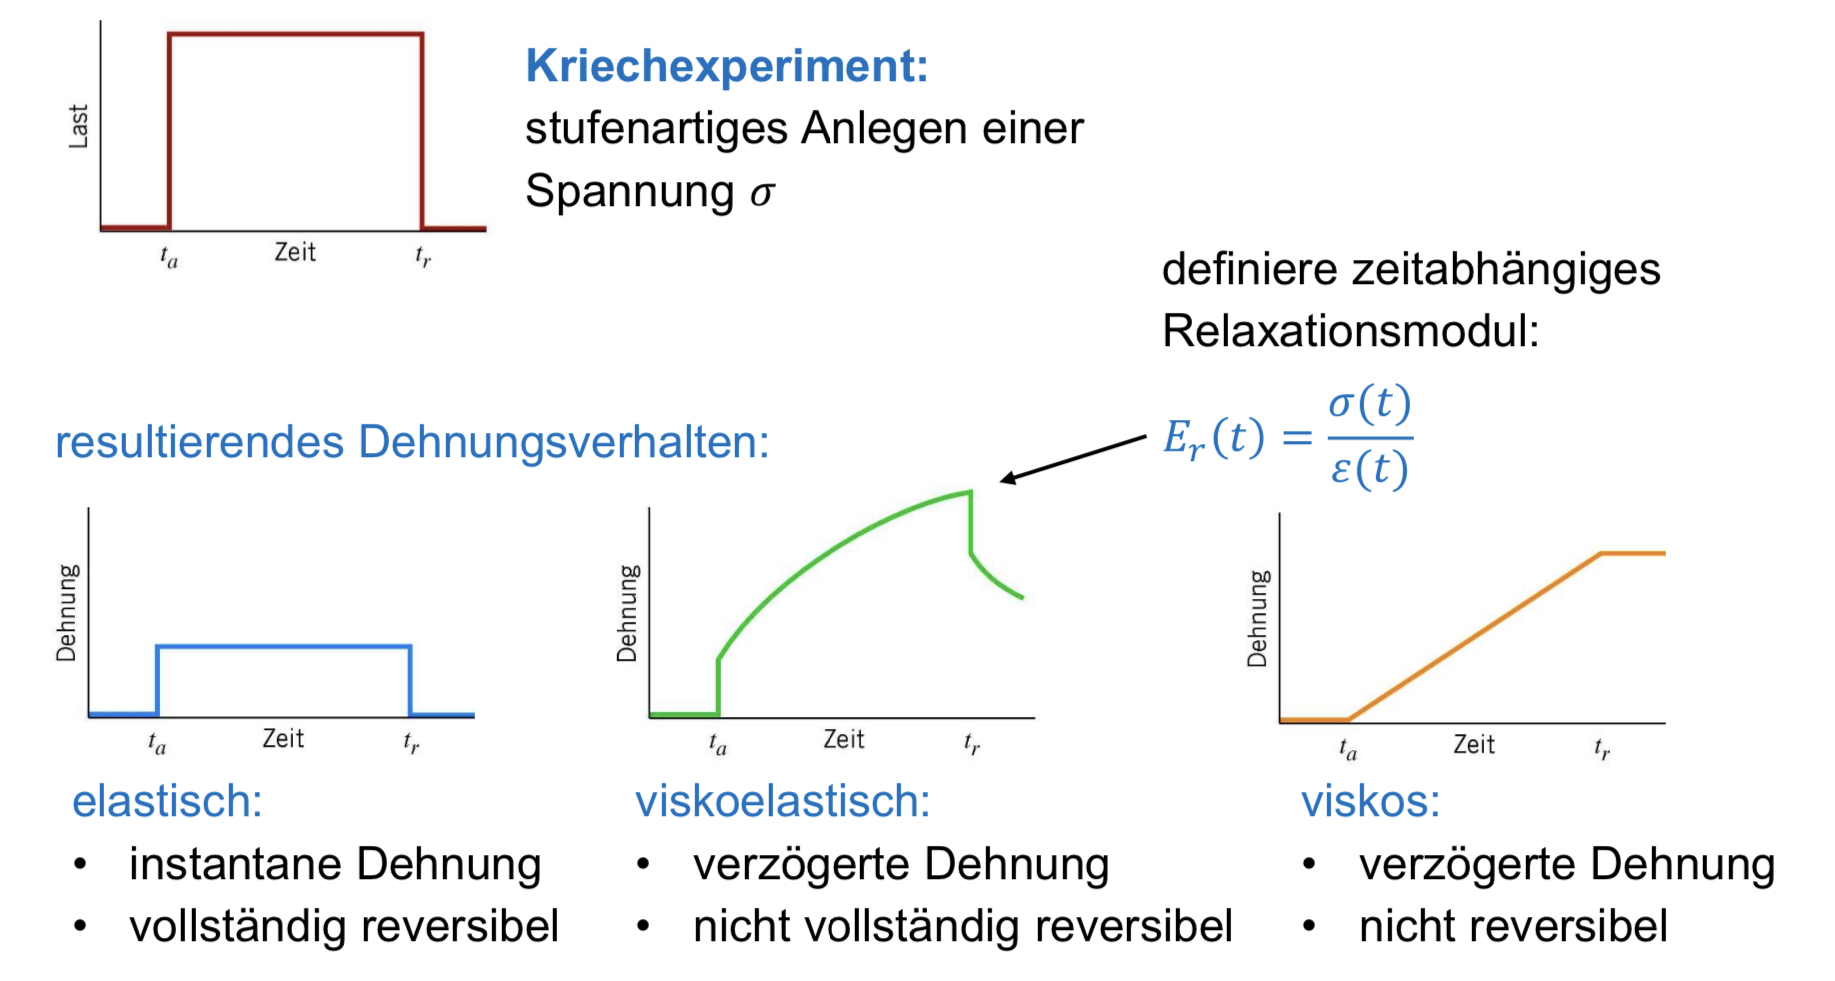
\includegraphics[width = \textwidth]{images/Materialwissenschaften/Kriechexperiment.jpeg}
    \caption{Verschiedene Dehnungsantworten auf eine stufenartige Spannung im Kriechexperiment}
    \label{fig:Kriechexperiment}
\end{figure}
Zum Anderen kann man das Relaxationsexperiment durchführen, dabei wird eine stufenartige Dehnung angelegt und die Spannungsantwort des Materials beobachtet, typische Spannungsantworten sind in Abbildung \ref{fig:Relaxationsexperiment} dargestellt.
\begin{figure}[h]
    \centering
    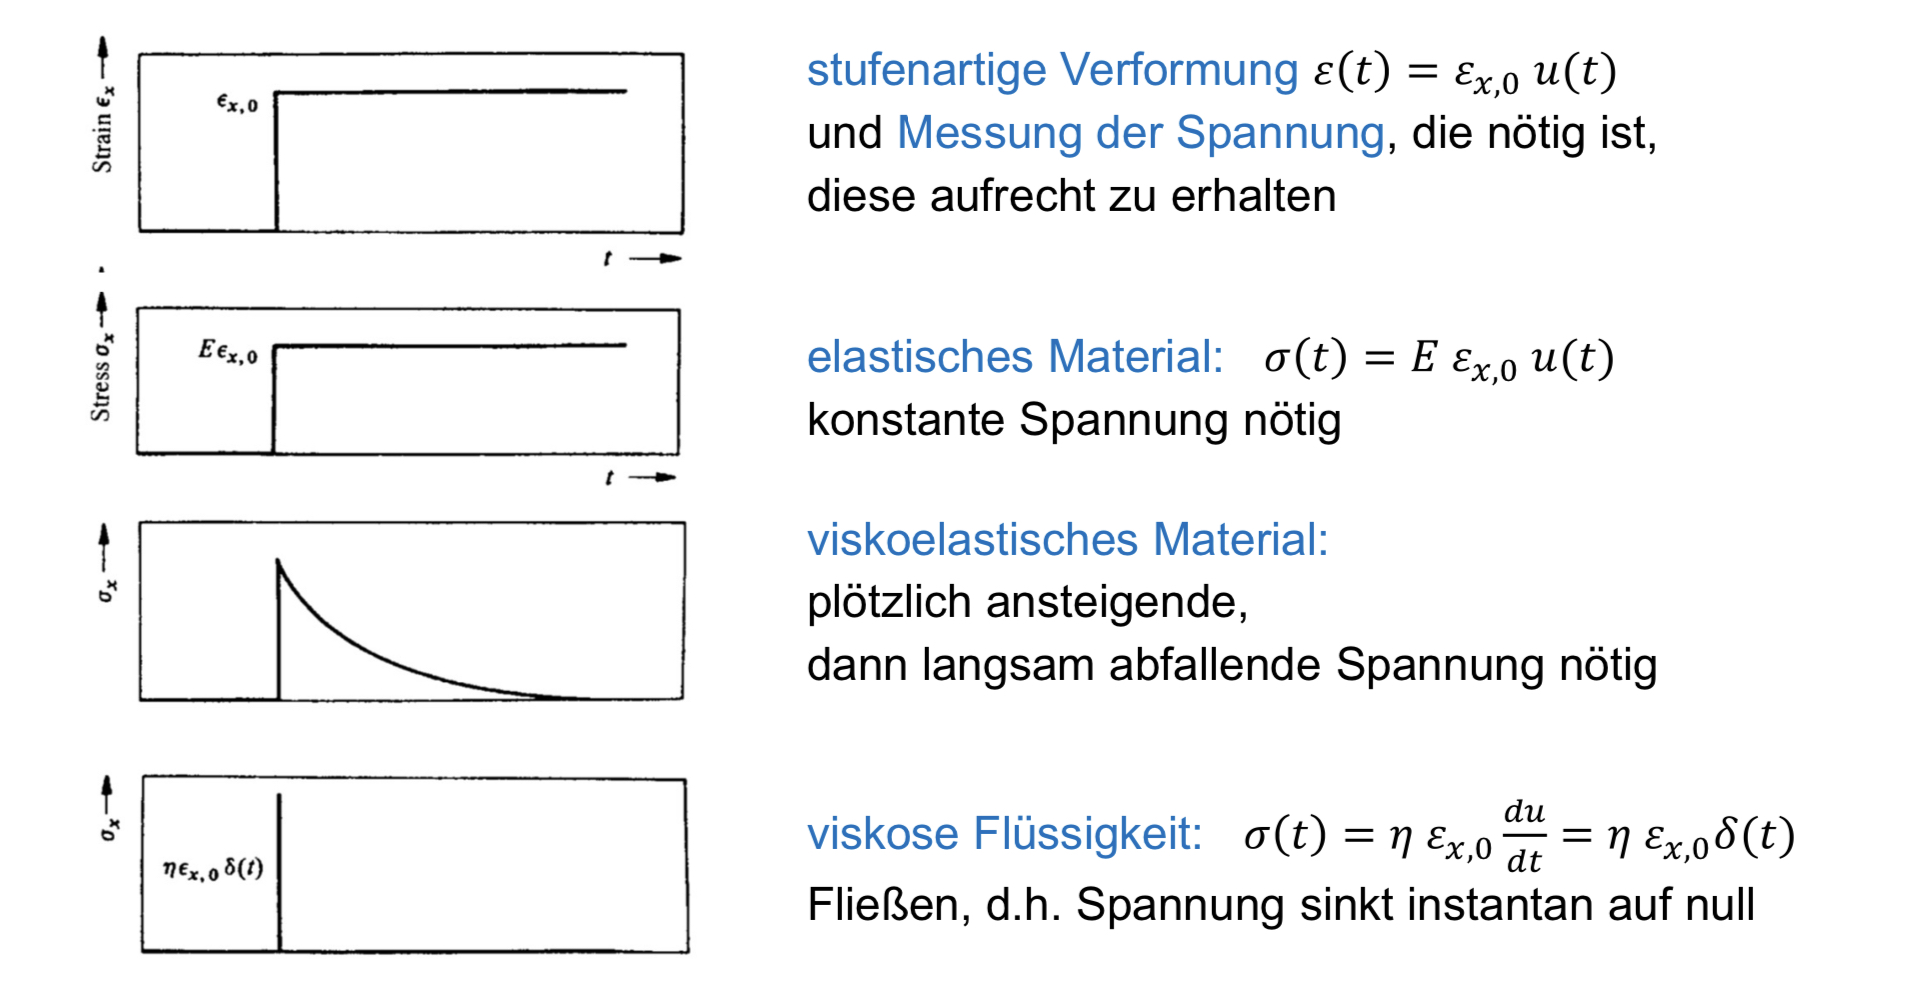
\includegraphics[width = 0.8\textwidth]{images/Materialwissenschaften/Relaxationsexperiment.jpeg}
    \caption{Verschiedene Spannungsantworten auf eine stufenartig angelegte Dehnung im Relaxationsexperiment}
    \label{fig:Relaxationsexperiment}
\end{figure}
\end{addmargin}

\noindent\textbf{3. Welche Gründe gibt es für viskoelastisches Verhalten?}\\
\begin{addmargin}[25pt]{0pt}
Viskoelastisches Verhalten basiert entweder auf thermischer Bewegung der Teilchen, das tritt häufig in Metallen und Keramiken auf, oder auf zahlreichen Relaxationsprozessen was in Polymerschmelzen oder komplexen Flüssigkeiten auftritt. \\
\end{addmargin}

\noindent\textbf{4. Welche mechanischen Bauelemente werden verwendet um viskoelastisches Verhalten zu modellieren?}\\
\begin{addmargin}[25pt]{0pt}
Um das rein elastische Verhalten in Festkörpern zu modellieren verwendet man eine Feder, damit kann man sehr präzisse das Hooke'sche Gesetz darstellen. Um eine reine viskose Flüssigkeit zu modellieren verwendet man einen Dämpfer.\\
\end{addmargin}

\noindent\textbf{5. Wie werden sie kombiniert und welche Arten von Verhalten können so modelliert werden?}\\
\begin{addmargin}[25pt]{0pt}
Um eine viskoelastische Flüssigkeit zu beschreiben verwendet man das Maxwell-Modell. In diesem Modell wird eine Feder mit einem Dämpfer in Reihe geschalten, dadurch verhält es auf kurze Zeiten elastisch und auf lange Zeiten viskos. Die Gesamtdehnung in diesem Modell ist die Summe der Einzeldehnungen. Für eine viskoelastischen Festkörper nutzt man das Voigt-Kelvin-Modell bei dem eine Feder und ein Dämpfer parallel geschalten sind. Hierbei ist die Spannung die Summe der Einzelspannungen. Auf kurze Zeit verhält dieses Modell viskos und auf lange Zeit elastisch, genau so wie man das von einem viskoelastischen Festkörper erwartet.\\
\end{addmargin}


\subsection{Mechanische Eigenschaften von Metallen}
\noindent\textbf{1. Wie äußert sich plastische Verformung im Spannungs-Dehnungs-Diagramm und durch welche Größen wird sie charakterisiert?}\\
\begin{addmargin}[25pt]{0pt}
\begin{figure}[h]
    \centering
    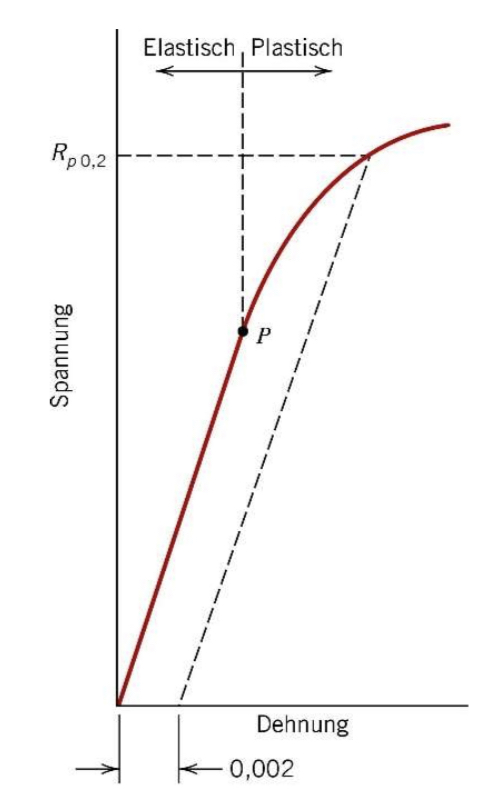
\includegraphics[width=0.5\textwidth]{images/Materialwissenschaften/plastische_Verformung.jpeg}
    \caption{Vergleich von elastischem und plastischem Bereich }
    \label{fig:plastische_Verformung}
\end{figure}
Bei sehr großen Dehnungen werden die Kristallstrukturen stark genug auseinander gezogen dass Bindungen reißen können, diesen Bereich nennt man Bereich der plastischen Verformung. Da einige Bindungen nun aufgebrochen sind ist der Widerstand des Werkstoffs gegenüber Verformung nicht mehr so stark und die Spannungs-Dehnungs-Kurve steigt flacher an als im elastischen Bereich (siehe Abbildung \ref{fig:plastische_Verformung}). Der Spannungswert ab dem es zu plastsischer Verformung kommt nennt sich Streckgrenze. Außerdem kann man die Ersatzstreckgrenze definieren, das ist die Spannung die sich aus dem Schnittpunkt der Spannungs-Dehnungs-Kurve mit einer zum linearen Bereich parallelen Gerade, welche bei $\epsilon = 0,002$ die Dehnungs-Achse schneidet, ergibt.\\
\end{addmargin}

\noindent\textbf{2. Wie sind die Zugfestigkeit und die Bruchfestigkeit definiert?}\\
\begin{addmargin}[25pt]{0pt}
    Die Zugfestigkeit ist der maximale Spannungswert eines Werkstoffs im Spannungs-Dehnungs-Diagramm. Dehnt man den Werkstoff noch weiter als diesen Punkt kommt es zur Einschnürung, dabei wird die Querschnittsfläche der Probe deutlich geringer und auch die Spannung nimmt dabei ab, dder Punkt an dem die Probe bricht ist dann typischerweise bei kleineren Spannungen als die Zugfestigkeit. Die Spannung zum Zeitpunkt des Drucks wird als Bruchfestigkeit bezeichnet.  \\
\end{addmargin}

\noindent\textbf{3. Wodurch unterscheiden sich die Spannungs-Dehnungskurven von spröden und duktilen Metallen?}\\
\begin{addmargin}[25pt]{0pt}
Spröde Materialien haben fast keine plastische Verformung bevor sie brechen wohingegen duktile Materialien erst sehr stark plastisch verformt werden bevor sie brechen. Dieser Sachverhalt ist in Abbildung \ref{fig:duktil_spröde} nochmal visualisiert.\\
\begin{figure}[h]
    \centering
    \includegraphics[width = 0.8\textwidth]{images/Materialwissenschaften/spröde_duktil_sigma_epsilon.jpeg}
    \caption{Unterschied der plastischen Verformung zwischen duktilen und spröden Werkstoffen}
    \label{fig:duktil_spröde}
\end{figure}
\end{addmargin}

\noindent\textbf{4. Was bedeutet Rückfederung und was ist der Rückfederungsmodul?}\\
\begin{addmargin}[25pt]{0pt}
Rückfederung nennt man den Prozess der im elastischen Bereich auftritt. Durch die Dehnung wird die Kristallstruktur gedehnt und somit Energie gespeichert. Diese Energie kann dann vollständig reversibel wieder abgegeben werden und der Probenkörper kehrt in seine ursprüngliche Form zurück. Zur Charakterisierung dieses Verhaltens nutzt man den Rückfederungsmodul $E_r$, welcher angibt wie viel Energie pro Volumeneinheit vom Kristall absorbiert wurde. Er ist definiert als die Fläche unter der Spannungs-Dehnungs-Kurve bis zur Streckgrenze $\sigma_y$: 
\begin{equation}\label{eq:Rückfederungsmodul}
    E_r = \int\limits_0^{\epsilon_y}\sigma\; \si{d}\epsilon = \frac{1}{2}\sigma_y\epsilon_y = \frac{\sigma_y^2}{2E}
\end{equation}
Das bedeutet, dass man für Federn ein Material verwenden sollte, welches einen niedrigen Elastizitätsmodul und eine hohe Streckgrenze besitzt damit der Rückfederungsmodul maximiert wird.\\
\end{addmargin}

\noindent\textbf{5. Was bedeutet Zähigkeit?}\\
\begin{addmargin}[25pt]{0pt}
Die Zähigkeit ist ein Maß für die Fähigkeit eines Materials vor dem Bruch Energie zu absorbieren und sich plastisch zu verformen. Zur quantitativen Beschreibung der Zähigkeit verwendet man die Fläche unter der Spannungs-Dehnungs-Kurve bis zum Bruch. Desto größer diese Fläche ist desto zäher ist ein Material. Daraus folgt auch direkt dass duktile Materialien im Normalfall deutlich zäher sind als spröde Materialien. \\
\end{addmargin}

\noindent\textbf{6. Was sind wahre Spannung und wahre Dehnung und wie ist der Verlauf der wahren Spannungs-Dehnungskurve für ein duktiles Metall?}\\
\begin{addmargin}[25pt]{0pt}
Die Spannung $\sigma$ wurde ursprünglich definiert als wirkende Kraft pro Fläche auf die diese Kraft wirkt. Dabei wurde angenommen, dass die Querschnittsfläche der Probe konstant bleibt. Das ist allerdings allgemein nicht der Fall wodurch es Sinn ergibt die wahre Spannung $\sigma_w$ als Kraft pro aktueller Querschnittsfläche $A_i$ zu definieren. Ebenso muss man die Dehnung auch anpassen es ergibt sich: 
\begin{align}\label{eq:wahre_Spannung}
    \sigma_w &= \frac{F}{A_i}\\\label{eq:wahre_Dehnung}
    \epsilon_w &= \int\limits_{l_0}^{l_i} \frac{\si{d}l}{l} = \ln \frac{l_i}{l_0}
\end{align}
Der Wert der praktischen Spannung ist praktisch, da er das intuitiv erwartete Verhalten, dass die Spannung oberhalb der Zugfestigkeit weiter steigt, aufweist. Bis Einschnürung auftritt kann man die wahre Spannung und Dehnung noch mit den technischen Größen $\sigma$ und $\epsilon$ in Verbindung setzen:
\begin{align}\label{eq:wahre_Spannung_mit_technischen_Größen}
    \sigma_w &= \sigma(1+\epsilon)\\ \label{eq:wahre_Dehnung_mit_technischen_Größen}
    \epsilon_w &= \ln (1+\epsilon)
\end{align}
\end{addmargin}

\noindent\textbf{7. Was ist elastische Erholung?}\\
\begin{addmargin}[25pt]{0pt}
Wenn ein Probenkörper über die Streckgrenze gedehnt wurde, dann treten plastische, irreversible Verformungen auf. Lässt man nun den Körper entspannen so wird er eine Dehnung aufweisen obwohl keine Spannung mehr anliegt. Diese Erholung des Materials geschieht auf einer Geraden parallel zum ursprünglichen elastischen Bereich. Falls man nun eine erneute Spannung an den bereits plastisch verformten Körper anlegt, so wird er wieder entlang dieser elastischen Geraden auf die Spannungs-Dehnungs-Kurve zurückkehren. Dieses Materialverhalten nennt man elastische Erholung.\\
\end{addmargin}

\noindent\textbf{8. Was ist Härte und wie wird sie gemessen?}\\
\begin{addmargin}[25pt]{0pt}
Die Härte ist ein Maß dafür wie stark der Widerstand eines Materials gegen lokale plastische Verformungen, wie ein kleiner Eindruck oder Ritz, ist. Die Härte ist eine schwer zu quantisierende Größe. Man misst die Härte indem man einen genormten Testkörper, den sogenannten Indenter, mit einer festen Prüfkraft und Prüfdauer in die Oberfläche des MAterials drückt und sich danach die Größe des Eindrucks anschaut.    \\
\end{addmargin}

\noindent\textbf{9. Welchen Effekt haben Schubspannungen auf Stufen -und Schraubenversetzungen?}\\
\begin{addmargin}[25pt]{0pt}
Durch Schubspannungen werden die Defekte an die Oberfläche des Körpers verschoben. Dabei werden bei Stufenversetzungen die Versetzungslinien parallel zur Schubspannung verschoben und bei Schraubenversetzungen senkrecht zur Schubspannung. \\
\end{addmargin}

\noindent\textbf{10. Was passiert bei Verformung an der Versetzungslinie einer Stufenversetzung?}\\
\begin{addmargin}[25pt]{0pt}
    An der Versetzungslinie kommt es zu einer Gitterverzerrung, da dort auf einer Seite eine Druckkraft und auf der anderen Seite eine Zugkraft wirkt. In einem idealen Kristallgitter kann es zu Versetzungsannihilation kommen. \\
\end{addmargin}

\noindent\textbf{11. Was sind Gleitsysteme?}\\
\begin{addmargin}[25pt]{0pt}
Gleitsysteme beschreiben allgemein in welche Richtung sich eine Versetzung bewegen wird. Ein Gleitsystem besteht dabei aus einer Gleitebene, das ist die dichtest gepackte Ebene und eine Gleitrichtung, das ist analog die dichtest gepackte Richtung. Das Gleitsystem ist die energetisch günstigste Variante Versetzungen zu bewegen weil dabei am wenigsten Atome auf neue Gitterplätze verschoben werden müssen.\\
\end{addmargin}

\noindent\textbf{12. Wie verformen sich Polykristalle plastisch?}\\
\begin{addmargin}[25pt]{0pt}
Da jedes Korn eine unterschiedliche Ausrichtung der Kristallstruktur hat variiert auch die Gleitrichtung von einem Korn zum Anderen. Die Körner und die Korngrenzen bleiben dabei intakt, lediglich die einzelnen Körner verformen sich. Falls Gleiten nicht möglich ist werden sich unter äußerer Spannung Zwillingsgrenzen bilden während sich Polykristalle plastisch verformen.\\
\end{addmargin}


\subsection{Mechanische Eigenschaften von Polymeren}
\noindent\textbf{1. Wie sind Polymere aufgebaut? Welche Architekturen kennen Sie?}\\
\begin{addmargin}[25pt]{0pt}
Polymere bestehen aus langen Ketten von Wiederholeinheiten, sogenannten Monomeren. Diese Ketten können entweder linear, verzweigt oder vernetzt angeordnet sein. Es ist auch nicht ausgeschlossen, dass ein Polymer aus mehreren Monomeren aufgebaut ist. Ein Polymer, welches nur eine Wiederholeinheit besitzt nennt man Homopolymer. Polymere mit mehreren Wiederholeinheiten sind als Copolymere bekannt. \\
\end{addmargin}

\noindent\textbf{2. Durch welche Kenngrößen werden einzelne Polymere charakterisiert?}\\
\begin{addmargin}[25pt]{0pt}
Polymere werden durch den Polymerisationsgrad DP und die Molmasse $M$ charakterisiert. Dabei gibt DP an wie lang die Polymerketten sind, also aus wie vielen Monomeren das Polymer besteht. Der Polymerisationsgrad liegt typischerweise zwischen 100 und 10000. Die Molmasse ist die molare Masse des Polymers, welche bestimmt wird aus der Masse des Monomers $M_{\si{mon}}$ und dem Polymerisationsgrad DP: $M = \si{DP} \cdot M_{\si{mon}}$. Die Eigenschaften des Polymer hängen dabei sehr stark von $M$ ab.  \\
\end{addmargin}

\noindent\textbf{3. Was sind Thermoplaste und wie ist ihr Temperaturverhalten?}\\
\begin{addmargin}[25pt]{0pt}
Thermoplaste sind Elastomere deren Eigenschaften stark von der Temperatur abhängen. Thermoplaste werden weicher bei Erhitzung und Erstarren beim Abkühlen. Dieser Prozess ist vollständig reversibel, das bedeutet man kann Thermoplaste Erhitzen, dann verformen und schließlich wieder abkühlen und hat schließlich ein festes, schwer verformbares Material in einer beliebigen Form. Man kann diesen Prozess beliebig häufig durchführen. \\
\end{addmargin}

\noindent\textbf{4. Was sind Duroplaste und wie ist ihr Temperaturverhalten?}\\
\begin{addmargin}[25pt]{0pt}
Duroplaste werden während der Verarbeitung irreversibel ausgehärtet. Dabei wird durch Temperaturerhöhung die Anzahl kovalenter Bindungen zwischen den Polymerketten sehr stark erhöht. Durch diese zusätzlichen Bindungen wird der Duroplast stabil aber lässt sich auch nicht mehr zurückformen. Duroplaste sind härter und stabiler als Thermoplaste.\\
\end{addmargin}

\noindent\textbf{5. Welche Arten von Copolymeren kennen Sie?}\\
\begin{addmargin}[25pt]{0pt}
Es gibt 3 Arten von Copolymeren. Die erste Art der Copolymere ist das statistische Copolymer, bei diesem sind die verschiedenen Monomere beliebig angeordnet und folgen keiner Ordnung. Außerdem gibt es noch das Blockpolymer, dabei findet man immer einen Block von Monomer A  gefolgt von einem Block von Monomer B. Die dritte Art der Copolymere ist das Pfropfcopolymer, dieses besteht aus einer langen Hauptkette von Monomer A und an dieser hängen Nebenketten bestehend aus Monomer B.\\
\end{addmargin}

\noindent\textbf{6. Wie sind die Ketten in kristallinen Bereichen angeordnet? Welche Form haben die Kristallite? Wie sind die Kristallite angeordnet?}\\
\begin{addmargin}[25pt]{0pt}
Im kristallinen Bereich von teilkristallinen Polymeren sind die Kettenstücke parallel angeordnet und gefaltet. Dadurch bilden sich 10 bis 20 Nanometer dünne Plättchen mit einer lateralen Ausdehnung von 10 bis 50 Mikrometer, diese Plättchen nennt man Kristallite. Kristallite ordnen sich zu Sphäroliten zusammen, das sind kugelförmige Objekte welche von einem Kristallkern aus wachsen. An diesen Kristallkern lagern sich mehrere Kristallite kettenartig an, in den Zwischenräumen zwischen den Kristallitketten bilden sich amorphe Bereiche. \\
\end{addmargin}

\noindent\textbf{7. Wie können Spannungs-Dehnungs-Kurven von Polymermaterialien aussehen?}\\
\begin{addmargin}[25pt]{0pt}
Poymere können eine Vielzahl von verschiedenen mechanischen Verhaltensweisen aufweisen, somit sind auch so ziemlich alle Spannungs-Dehnungs-Kurven vorstellbar. Die häufigsten auftretenden Kurven sind die des spröden Materials, die des plastischen Materials und die des Elastomers. Das spröde Material kennzeichnet sich durch einen hohen Elastizitätsmodul im elastischen Bereich und danach bricht das Material direkt ohne sich plastisch zu verformen. Das plastische Material hingegen weist nach der elastischen Dehnung ein Fließverhalten auf bevor es zum Bruch kommt. Ein Elastomer lässt sich vollständig elastisch deformieren.\\
\end{addmargin}

\noindent\textbf{8. Wie hängen die mechanischen Eigenschaften von Polymermaterialien von der Temperatur ab?}\\
\begin{addmargin}[25pt]{0pt}
Die Temperatur hat einen sehr großen Einfluss auf die mechanischen Eigenschaften des Polymers. Eine höhere Temperatur erleichtert es ein Material zu verformen, wodurch bei höheren Temperaturen allgemein der Elastizitätsmodul und die Zugfestigkeit niedriger sind. \\
\end{addmargin}

\noindent\textbf{9. Welche Rolle spielt die Zeit für den Elastizitätsmodul? Wie ist der Relaxationsmodul definiert?}\\
\begin{addmargin}[25pt]{0pt}
Viskoelastische Polymermaterialien weisen ein stark temperatur- und zeitabhängiges Verhalten auf. Bei ihnen nimmt der Elastizitätsmodul mit der Zeit ab, wenn man instantan eine konstante Dehnung $\epsilon_0$ anlegt. Diese Zeitabhängigkeit wird durch den Relaxationsmodul $E_r$ beschrieben:
\begin{equation}\label{eq:Relaxationsmodul}
    E_r(t) = \frac{\sigma (t)}{\epsilon_0}
\end{equation}
Der Relaxationsmodul hängt ebenfalls von der Temperatur ab, da eine höhere Temperatur die Fließeigenschaften des Materials begünstigt sinkt $E_r$ mit steigender Temperatur.\\
\end{addmargin}

\noindent\textbf{10. Wie wird eine Masterkurve konstruiert und was kann man an ihr ablesen?}\\
\begin{addmargin}[25pt]{0pt}
\begin{figure}[h]
    \centering
    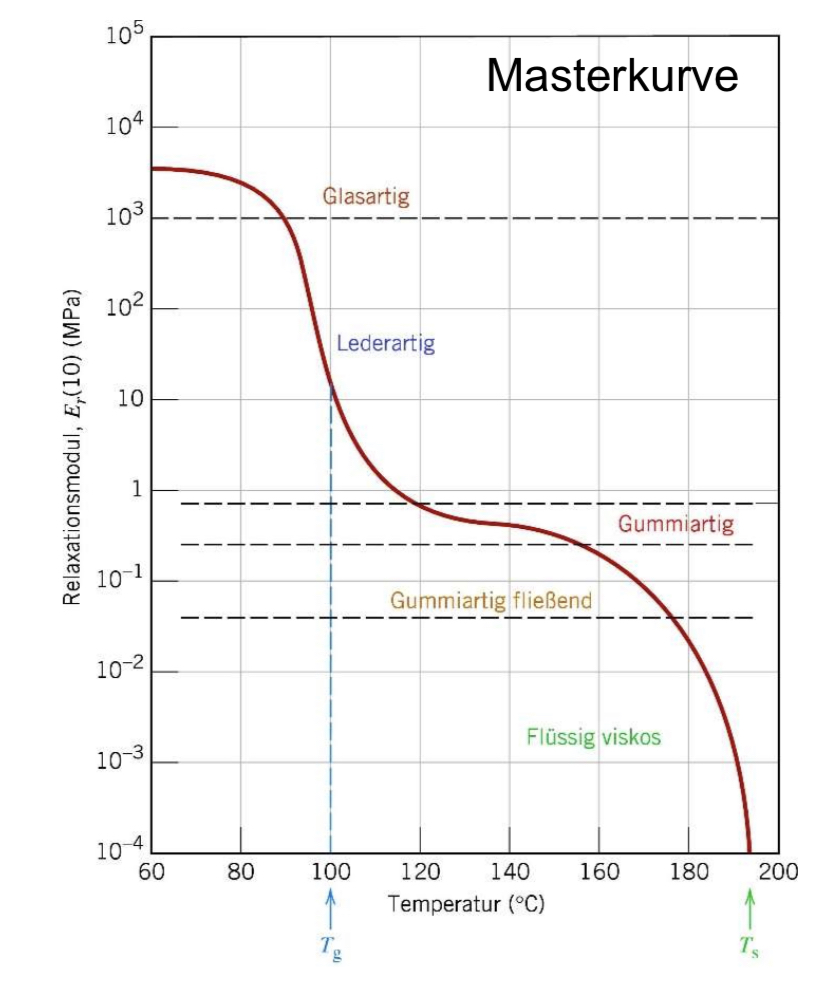
\includegraphics[width = 0.8\textwidth]{images/Materialwissenschaften/Masterkurve.jpeg}
    \caption{Beispiel einer Masterkurve mit den verschiedenen Bereichen für glasartig, gummiartig und fließend viskos}
    \label{fig:Masterkurve}
\end{figure}
Bei der Masterkurve wird der Relaxationsmodul gegen die Temperatur aufgetragen, dabei kann man dann ablesen im welchem Temperaturbereich das Material sich wie verhält. In Abbildung \ref{fig:Masterkurve} ist diese für amorphes Polystyrol beispielhaft dargestellt. Mit $T_g$ wird die Glasübergangstemperatur bezeichnet, das ist die Temperatur bei der das Verhalten des Glases von lederartig zu glasartig übergeht. $T_s$ ist die Schmelztemperatur, da geht der Relaxationsmodul gegen null.\\
\end{addmargin}

\noindent\textbf{11. Was passiert beim Dehnen von Elastomeren?}\\
\begin{addmargin}[25pt]{0pt}
Die gefalteten langen Polymerketten falten sich auf und es liegen geradlinige Ketten vor, dadurch kann sich das Material sehr gut in Zugrichtung elastisch dehnen. Dabei wird die Entropie verringert, da das System nun geordneter vorliegt. Außerdem wird das Elastomer warm beim Dehnen da man Energie in das Material reinsteckt und nur ein Teil davon benötigt wird um die Entropie zu verringern. Die gesamte innere Energie des Systems erhöht sich.\\
\end{addmargin}

\noindent\textbf{12. Was passiert beim Dehnen teilkristalliner Polymere makroskopisch und molekular?}\\
\begin{addmargin}[25pt]{0pt}
An oberer Fließgrenze kommt es zu Einschnürung, diese wird mit der Zeit verlängert. Dieses makroskopische Verhalten hat mehrere mikroskopische Gründe. Beim Dehnen werden die amorphen Ketten gestreckt und die Kristallite dicker. Bei starker Deformation werden die Kristallite aufbrechen und sich ausrichten.\\
\end{addmargin}

\subsection{Werkstoffversagen}
\noindent\textbf{1. Wie brechen spröde und duktile Materialien?}\\
\begin{addmargin}[25pt]{0pt}
Spröde Materialien brechen ohne sich vorher plastisch zu verformen wohingegen duktile Materialien erst sehr stark plastisch verformt werden bevor es zu einem Bruch kommt. Dieser Sachverhalt ist in Abbildung \ref{fig:duktil_spröde} visualisiert.\\
\end{addmargin}

\noindent\textbf{2. Wie sehen die Bruchflächen aus beim überwiegend duktilem Bruch, mäßig duktilem Bruch und beim Sprödbruch?}\\
\begin{addmargin}[25pt]{0pt}
Bei einem überwiegend duktilem Bruch kommt es im Bereich der plastischen Verformung zu Einschnürung bis der Querschnitt punktförmig ist, ersst an diesem Punkt bricht das Material. Reißt man ein duktiles Material an einer Stelle ein so verlängert sich dieser Riss nur wenn man die einwirkende Spannung erhöht, diese Art von Riss nennt man stabilen Riss. Ein mäßig duktiler Bruch hat keine extreme Einschnürung, bei ihm kommt es lediglich zu einer geringen Einschnürung bevor kleine Hohlräume gebildet werden die mit steigender Spannung immer größer werden und schließlich einen elliptischen Riss verursachen. Das andere Extrem zum duktilen Bruch ist der Sprödbruch, bei diesem kommt es zu keiner Einschnürung und es entsteht ein Riss senkrecht zur Zugrichtung mit einer flachen Bruchkante. Die 3 Arten des Bruchs sind in Abbildung \ref{fig:Brucharten} dargestellt.\\
\begin{figure}[h]
    \centering
    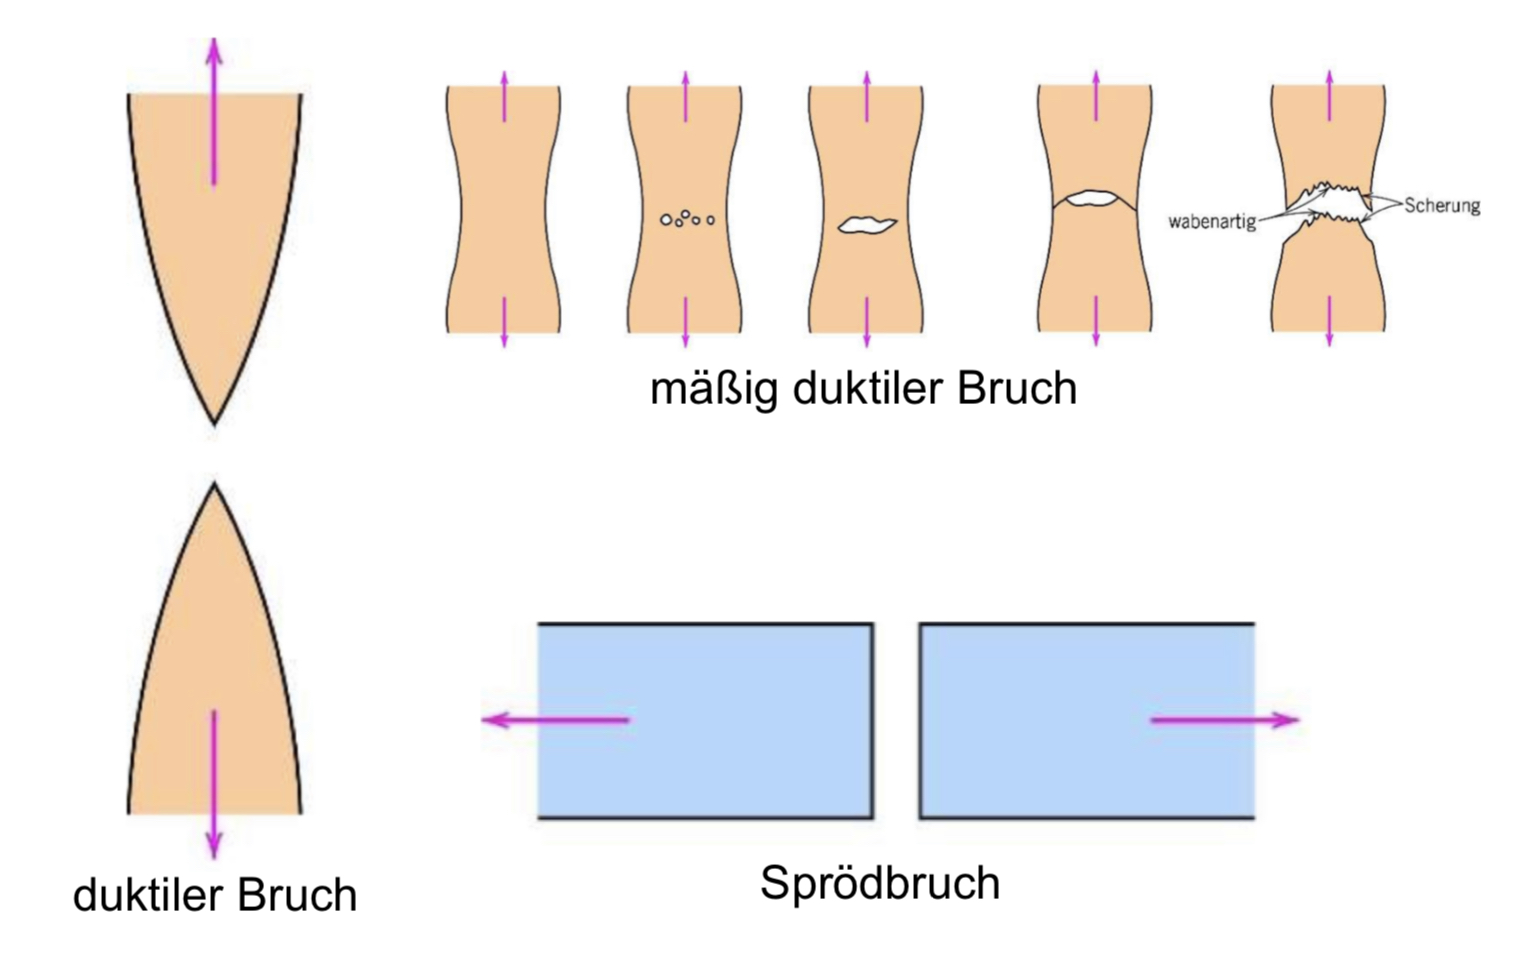
\includegraphics[width = 0.8\textwidth]{images/Materialwissenschaften/Brucharten.jpeg}
    \caption{Visualisierung der 3 Arten des Bruchs, links sieht man den duktilen Bruch, rechts oben den mäßig duktilen Bruch und rechts unten den Sprödbruch.}
    \label{fig:Brucharten}
\end{figure}
\end{addmargin}

\noindent\textbf{3. Auf welche Arten können Risse in polykristallinen Materialien ausbreiten?}\\
\begin{addmargin}[25pt]{0pt}
In polykristallinen Materialien kann es entweder zu einem transgranularem Bruch oder einem intergranularem Bruch kommen. Bei dem transgranularem Bruch breitet sich der Riss unabhängig von den Korngrenzen durch die Körner hindurch aus. Der Riss verläuft entlang spezifischer kristallografischer Ebenen. Beim intergranularem Bruch breitet sich der Riss entlang der Korngrenzen aus, diese Art des Risses entsteht wenn Korngrenzen geschwächt oder versprödet sind. In Abbildung \ref{fig:Rissausbreitung_polykristallin} sind die beiden Rissarten visualisiert.\\
\begin{figure}[h]
    \centering
    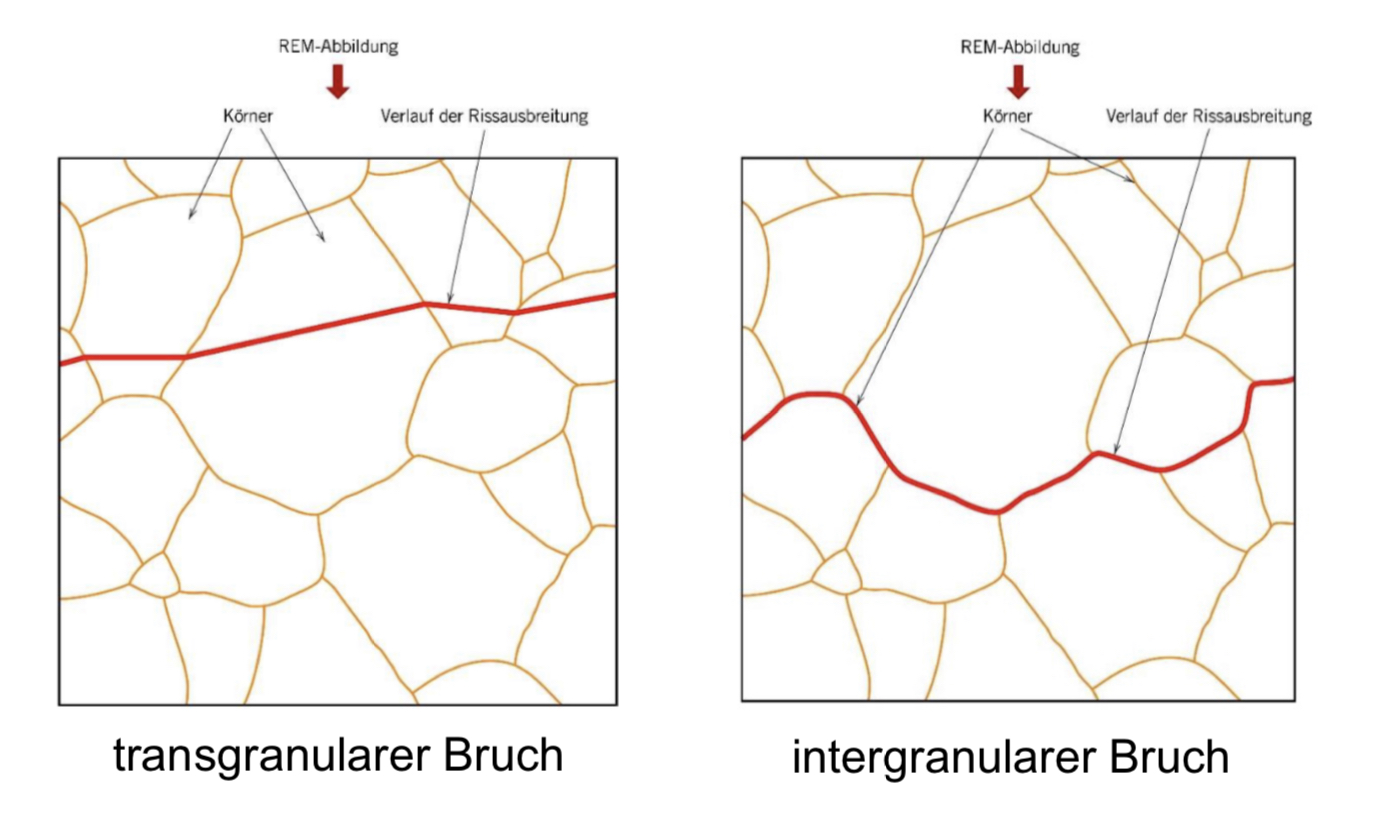
\includegraphics[width = 0.75\textwidth]{images/Materialwissenschaften/Rissausbreitung_polykristallin.jpeg}
    \caption{Darstellung der 2 Arten der Rissausbreitung in polykristallinen Materialien, links der transgrnulare Bruch und recht der intergranulare Bruch.}
    \label{fig:Rissausbreitung_polykristallin}
\end{figure}
\end{addmargin}

\noindent\textbf{4. Wie verhält sich die Spannung an einer Riss-Spitze?}\\
\begin{addmargin}[25pt]{0pt}
An einer Rissspitze kommt es zu einer lokalen Spannungsüberhöhung, das bedeutet, dass dort die Spannung $\sigma_m$ deutlich höher ist als die nominal anliegende Spannung $\sigma_0$:
\begin{equation}\label{eq:Spannung_Rissspitze}
\sigma_m = 2\sigma_0 \left( \frac{a}{\rho_t}\right)^\frac{1}{2}
\end{equation}
wobei $a$ die halbe Länge des inneren, elliptischen Risses ist und $\rho_t$ der Krümmungsradius an der Riss-Spitze. Der Faktor $\frac{a}{\rho_t}$ kann sehr hohe Werte annehmen für einen langen dünnen Riss.\\
\end{addmargin}

\noindent\textbf{5. Von was hängt die Bruchzähigkeit ab und welche Werte nimmt sie für spröde und duktile Materialien an?}\\
\begin{addmargin}[25pt]{0pt}
Die Bruchzähigkeit $K_c$ ist definiert als:
\begin{equation}\label{eq:definition_Bruchzähigkeit}
    K_c = Y\sigma_c \sqrt{\pi a}
\end{equation}
dabei ist $Y$ ein dimensionsloser Parameter, welcher die Geometrie des Risses und des Bauteils sowie die Art der Belastung beinhaltet, $\sigma_c$ ist die kritische Spannung für die Ausbreitung eines Risses in einem spröden Material und ist definiert als:
\begin{equation}\label{eq:definition_kritische_Spannung_sprödes_Material}
    \sigma_c = \left( \frac{2E\gamma_s}{\pi a}\right)^\frac{1}{2}
\end{equation}
dabei ist $E$ der Elastizitätsmodul und $\gamma_s$ die spezifische Bruchflächenenergie. Bei Beanspruchung nach Mode I, das ist eine Öffnungs- oder Zugbeanspruchung, ist die Bruchzähigkeit für spröde Materialien niedrig und für duktile Materialien hoch.\\
\end{addmargin}

\noindent\textbf{6. Auf welche Arten können sich Risse ausbreiten?}\\
\begin{addmargin}[25pt]{0pt}
Ein Riss kann entweder stabil sein, das tritt ein wenn die anliegende Spannung $\sigma$ kleiner ist als die kritische Spannung $\sigma_c$, oder instabil wenn $\sigma > \sigma_c$. Der stabile Riss breitet sich nicht von alleine weiter aus sondern breitet sich langsam aus wenn die Spannung erhöht wird. Der instabile Riss breitet sich extrem schnell aus.\\
\end{addmargin}

\noindent\textbf{7. Von welchen Parametern hängt die kritische Spannung ab?}\\
\begin{addmargin}[25pt]{0pt}
Die kritische Spannung wurde bereits in Gleichung \ref{eq:definition_kritische_Spannung_sprödes_Material} definiert. Sie hängt von der spezifischen Bruchflächenenergie $\gamma_s$, dem Elastizitätsmodul $E$ und der halben Risslänge $a$ ab. Eine alternative Formulierung der kritischen Spannung ist:
\begin{equation}\label{eq:kritische_Spannung_alternativ}
    \sigma_c = \sqrt{\frac{2\gamma}{\pi l }}
\end{equation}
Dabei ist $\gamma$ die Oberflächenspannung und $l$ die Risslänge.\\
\end{addmargin}

\noindent\textbf{8. Welche Prozesse spielen beim duktilen Bruch eine Rolle?}\\
\begin{addmargin}[25pt]{0pt}
Duktile Brüche basieren mikroskopisch auf 2 Prozessen. Der erste Prozess ist die Bewegung von Versetzungen aufgrund der wirkenden Spannung. Der zweite Prozess ist die plastische Verformung bei der Bindungen zwischen den Atomen aufbrechen, durch diese gebrochenen Bindungen vor der Rissspitze kann sich der Riss entlang dieser gebrochenen Bindungen ausbreiten.\\
\end{addmargin}

\noindent\textbf{9. Wie kann die Schlagzähigkeit spröder Polymermaterialien erhöht werden?}\\
\begin{addmargin}[25pt]{0pt}
Durch Einbettung gummiartiger Partikel in glasförmige Polymere wird die Schlagzähigkeit erhöht. Gummiartige Partikel brechen duktil dadurch kann ein großer Teil der Verformungsenergie absorbiert werden, ohne dass das spröde Material direkt bricht. Sollte sich ein Riss durch den spröden Teil des Polymers ausbreiten und dann auf ein gummiartiges Partikel stoßen so wird dieser Riss gestoppt und das Material kann insgesamt höherer Belastung standhalten. \\
\end{addmargin}

\subsection{Phasendiagramme}
\noindent\textbf{1. Was ist die Löslichkeitsgrenze?}\\
\begin{addmargin}[25pt]{0pt}
Die Löslichkeitsgrenze gibt die maximale Konzentration gelöster Atome in einer anderen Substanz an. Im Folgenden wird das Beispiel Zucker löst sich in Wasser verwendet. Genau an der Löslichkeitsgrenze finden wir eine gesättigte Lösung vor. Fügt man nun noch mehr Zucker in die Lösung hinzu so kann dieser nicht mehr gelöst werden und es liegt ein 2-Phasengebiet aus kristallinen Zucker und der flüssigen Wasser-Zucker-Lösung vor. Die Löslichkeitsgrenze ist temperaturabhängig, desto höher die Temperatur des Systems ist, desto mehr Zucker kann in ihm gelöst werden.  \\
\end{addmargin}


\noindent\textbf{2. Was ist ein Phasengleichgewicht?}\\
\begin{addmargin}[25pt]{0pt}
Ein Phasengleichgewicht beschreibt den Zustand, dass 2 Phasen koexistieren und das System stabil ist, sich also zeitlich nicht ändert solange keine externen Faktoren es dazu zwingen. Im Phasengleichgewicht befindet sich das System an einem Minimum der freien Enthalpie.\\
\end{addmargin}


\noindent\textbf{3. Was ist ein Tripelpunkt?}\\
\begin{addmargin}[25pt]{0pt}
Ein Tripelpunkt ist der Punkt im Phasendiagramm eines einkomponentigen Systems an dem alle 3 Phasen, fest, flüssig und gasförmig gleichzeitig auftreten und miteinander im Gleichgewicht stehen. Der Tripelpunkt ist exakt beschrieben durch ein Wertepaar aus einer Temperatur und einem Druck. Am Tripelpunkt hat das System also keinen Freiheitsgrad, da alle thermodynamischen Variablen exakt bestimmt sind. Stehen nur 2 Phasen miteinander im Gleichgewicht so hat das System einen Freiheitsgrad, es gibt also für jede beliebige Temperatur genau einen Druck an dem die beiden Phasen im Gleichgewicht stehen können.\\
\end{addmargin}


\noindent\textbf{4. Wie sieht das Phasendiagramm eines binären isomorphen Systems aus?}\\
\begin{addmargin}[25pt]{0pt}
Das Phasendiagramm eines binär isomorphen Systems ist in Abbildung \ref{fig:Phasendiagramm_binar_isomorph} dargestellt. Ein binär isomorphes System besteht aus 2 Komponenten, in der Abbildung sind das Kupfer und Nickel. Isomorph bedeutet, dass beide Komponenten sich gut mischen, sowohl im flüssigen als auch im festen Zustand. Die beiden Atomsorten sind im festen Zustand nur gut mischbar wenn ihre Gitterstrukturen gleich sind, sie ähnliche Atomradien haben und sie nicht dazu neigen eine Verbindung einzugehen. Durch die gute Mischbarkeit gibt es nur eine Art der Kristallbildung in der sich dann je nach Zusammensetzung mehr Kupfer oder mehr Nickel befindet. Im Phasendiagramm ist die Zusammensetzung der Mischung gegen die Temperatur aufgetragen, im Diagramm sind dann die Solidus- und die Liquiduslinie eingezeichnet. Unterhalb der Soliduslinie sind nur feste Kristalle möglich, oberhalb der Liquiduslinie nur flüssige Schmelze. Im Bereich zwischen Solidus- und Liquiduslinie können sowohl Schmelze als auch feste Kristalle auftreten, diese Bereich nennt man 2-Phasenbereich.\\
\begin{figure}[h]
    \centering
    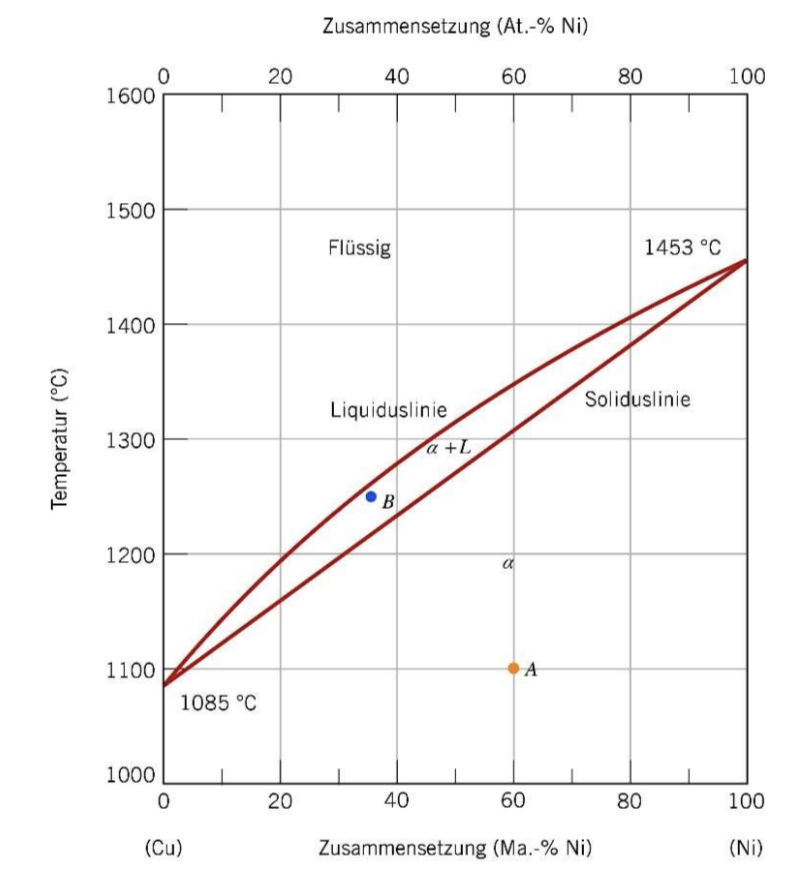
\includegraphics[width = 0.8\textwidth]{images/Materialwissenschaften/Phasendiagramm_binar_isomorph.jpeg}
    \caption{Phasendiagramm eines binär isomorphen System, hier am Beispiel von Kupfer-Nickel}
    \label{fig:Phasendiagramm_binar_isomorph}
\end{figure}
\end{addmargin}


\noindent\textbf{5. Wie verläuft das Schmelzen von Legierungen? }\\
\begin{addmargin}[25pt]{0pt}
Das Schmelzen einer festen Legierung beginnt ab der Soliduslinie. Für eine Mischung aus $50\%$ Kupfer und $50\%$ Nickel wäre das ab $1280^\circ \si{C}$. Danach befinden sich Schmelze und Kristall im Gleichgewicht, allerdings nimmt mit steigender Temperatur der Anteil an Schmelze im Gemisch zu bis dann an der Liquiduslinie reine Schmelze vorliegt. Bei der erwähnten Mischung von Kupfer und Nickel ist das bei ungefähr $1320^\circ \si{C}$ der Fall. \\
\end{addmargin}

\noindent\textbf{6. Wie kann die Zusammensetzung der Phasen
im Zweiphasengebiet bestimmt werden?}\\
\begin{addmargin}[25pt]{0pt}
\begin{figure}[h]
    \centering
    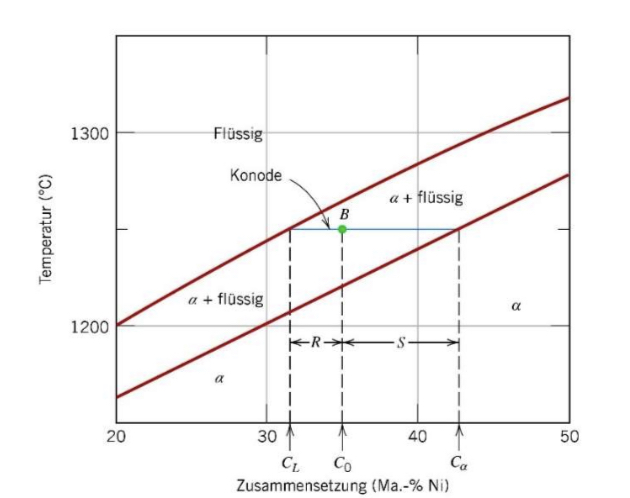
\includegraphics[width = 0.8\textwidth]{images/Materialwissenschaften/Zweiphasengebiet_Konode.jpeg}
    \caption{Das Zweiphasengebiet mit den Konoden $R$ und $S$ zur Bestimmung der Zusammensetzung von Schmelze und Kristall bzw. zur Bestimmung der Mengenanteile der Phasen.}
    \label{fig:zweiphasengebiet_konode}
\end{figure}
In Abbildung \ref{fig:zweiphasengebiet_konode} ist ein Punkt B im Zwei-Phasen-Gebiet eines Phasendiagramms dargestellt. Um die Zusammensetzung der Phasen zu bestimmen nutzt man Konoden, das sind Isothermen im Zweiphasengebiet. Die Schnittpunkte dieser Konoden mit der Solidus- bzw. Liquiduslinie geben die Zusammensetzung der festen bzw. flüssigen Phase an. In diesem Beispiel enthält die feste Phase $C_\alpha \approx 42,5\%$  Nickel wohingegen die flüssige Phase nur $C_L \approx 31,5\%$ Nickel enthält.\\
\end{addmargin}

\noindent\textbf{7. Wie können die Mengenanteile der Phasen
im Zweiphasengebiet bestimmt werden?}\\
\begin{addmargin}[25pt]{0pt}
Aus Abbidung \ref{fig:zweiphasengebiet_konode} kann man nicht nur die Zusammensetzung der Phasen bestimmen sondern auch wie viel der jeweiligen Phase im System vorhanden ist, dafür bestimmt man die Längen der Konoden und nennt diese $R$ und $S$ diese sind auch in Abbildung \ref{fig:zweiphasengebiet_konode} illustriert. Die Massenanteile an fester/flüssiger Phase sind dann:
\begin{align}
    Ma_\alpha &= \frac{R}{R+S}\\
    Ma_L &= \frac{S}{R+S}
\end{align}
Aus dieser und der letzten Frage ergibt sich noch eine interessante Erkenntnis, die Zusammensetzung der Phasen ist nur temperaturabhängig, also wenn man den Punkt B bei gleicher Temperatur nach links oder rechts verschiebt wird sich die Menge an Nickel in fester bzw. flüssiger Phase nicht ändern. Da sich bei einer Verschiebung nach rechts oder links $R$ und $S$ deutlich ändern werden sich die Massenanteile von flüssiger und fester Phase erheblich ändern. Das bedeutet, wenn man bei gleicher Temperatur 2 Kupfer-Nickel-Legierungen (mit unterschiedlichem Nickelgehalt) im Zweiphasengebiet beobachtet so haben die Schmelzen und die Kristalle jeweils genauso viel Nickel allerdings wird bei der Legierung mit dem insgesamt höheren Nickelanteil deutlich mehr feste Phase vorliegen.\\  
\end{addmargin}

\noindent\textbf{8. Wie kann das Phasendiagramm eines zweikomponentigen Systems 
aus der freien Mischungsenthalpie konstruiert werden?}\\
\begin{addmargin}[25pt]{0pt}
Man muss die freie Enthalpie für verschiedene Temperaturen, wie in Abbildung \ref{fig:Mischungsenthalpie_Phasendiagramm}, gegen die Zusammensetzung auftragen. Sollte die freie Enthalpie für alle Zusammensetzungen für eine Phase kleiner sein, dann befindet man sich im Einphasengebiet dieser Phase. Das Zweiphasengebiet erkennt man daran, dass sich die freien Enthalpien bei diesen schneiden, in Abbildung \ref{fig:Mischungsenthalpie_Phasendiagramm} ist das bei $T_3$ und $T_4$ der Fall. In diesem Fall muss man noch die eine Tangente finden, welche sowohl für die feste als auch für die flüssige Phasen eine Tangente ist. Die Schnittpunkte dieser Tangente mit den freien Enthalpien geben einem dann die Molzusammensetzungen der Solidus- und Liquiduslinie bei der bestimmten Temperatur an.\\
\begin{figure}[h]
    \centering
    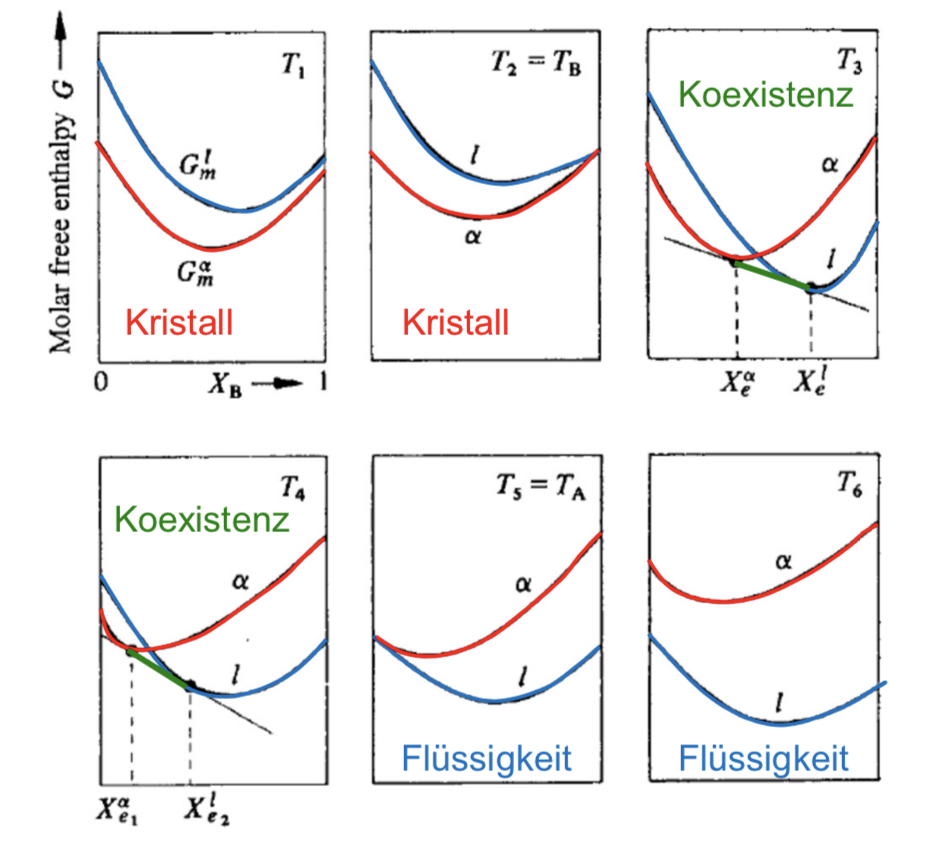
\includegraphics[width = 0.8\textwidth]{images/Materialwissenschaften/Mischungsenthalpie_Phasendiagramm.jpeg}
    \caption{Die freie Enthalpie in Abhängigkeit von der Zusammensetzung für verschiedene Temperaturen zur Bestimmung des Phasendiagramms.}
    \label{fig:Mischungsenthalpie_Phasendiagramm}
\end{figure}
\end{addmargin}

\noindent\textbf{9. Wie entsteht die Mikrostruktur in isomorphen Legierungen?}\\
\begin{addmargin}[25pt]{0pt}
Bei der Abkühlung einer Schmelze mit bestimmter Zusammensetzung tritt Keimbildung ab der Liquiduslinie ein. Dort bilden sich dann mehrere kleine Kristallkeime der festen Phase, welche mit sinkender Temperatur weiter wachsen. Bei der Soliduslinie ist die gesamte Schmelze erstarrt. Da es mehrere Keimzentren gab, welche alle gewachsen sind befinden sich nun Korngrenzen im Kristall. \\
\end{addmargin}

\noindent\textbf{10. Wie verhält sich die freie Mischungsenthalpie für Systeme mit einer Mischungslücke mit der Temperatur und wie sieht das zugehörige Phasendiagramm aus?}\\
\begin{addmargin}[25pt]{0pt}
Die freie Mischungsenthalpie für Systeme mit einer Mischungslücke ist stark temperaturabhängig. Bei hohen Temperaturen hat die freie Enthalpie nur ein Minimum, bei niedrigen Temperaturen hat die freie Mischungsenthalpie zwei Minima und dazwischen ein Maximum. die Temperatur bei der der Übergang zwischen diesen beiden charakteristischen Formen auftritt nennt man kritische Temperatur $T_c$. Im Phasendiagramm gibt es oberhalb der kritischen Temperatur nur eine Phase und unterhalb gibt es in einem gewissen Bereich ein Zweiphasengebiet. \\
\end{addmargin}

\noindent\textbf{11. Was ist charakteristisch für die Phasendiagramme eutektischer Systeme?}\\
\begin{addmargin}[25pt]{0pt}
Ein Phasendiagramm eines binären eutektischen Systems ist in Abbildung \ref{fig:Phasendiagramm_eutektisch} gezeigt. Eutektische Systeme zeichnen sich dadurch aus, dass sie 3 Phasen besitzen, zwei feste und eine flüssige. Die festen Phasen sind hier $\alpha$ und $\beta$ und die flüssige Phase wird als $L$ bezeichnet. Da es 3 Phasen gibt, existieren auch 3 Zweiphasengebiete. Ein weiteres Merkmal von eutektischen Systemen ist, dass die Schmelztemperatur der reinen Materialien höher ist als der Legierungen, die geringste Schmelztemperatur tritt am eutektischen Punkt $E$ auf. An diesem Punkt wird bei konstanter Temperatur die gesamte Schmelze in die beiden festen Phasen umgewandelt. Es gibt kein Dreiphasengebiet.\\   
\begin{figure}[h]
    \centering
    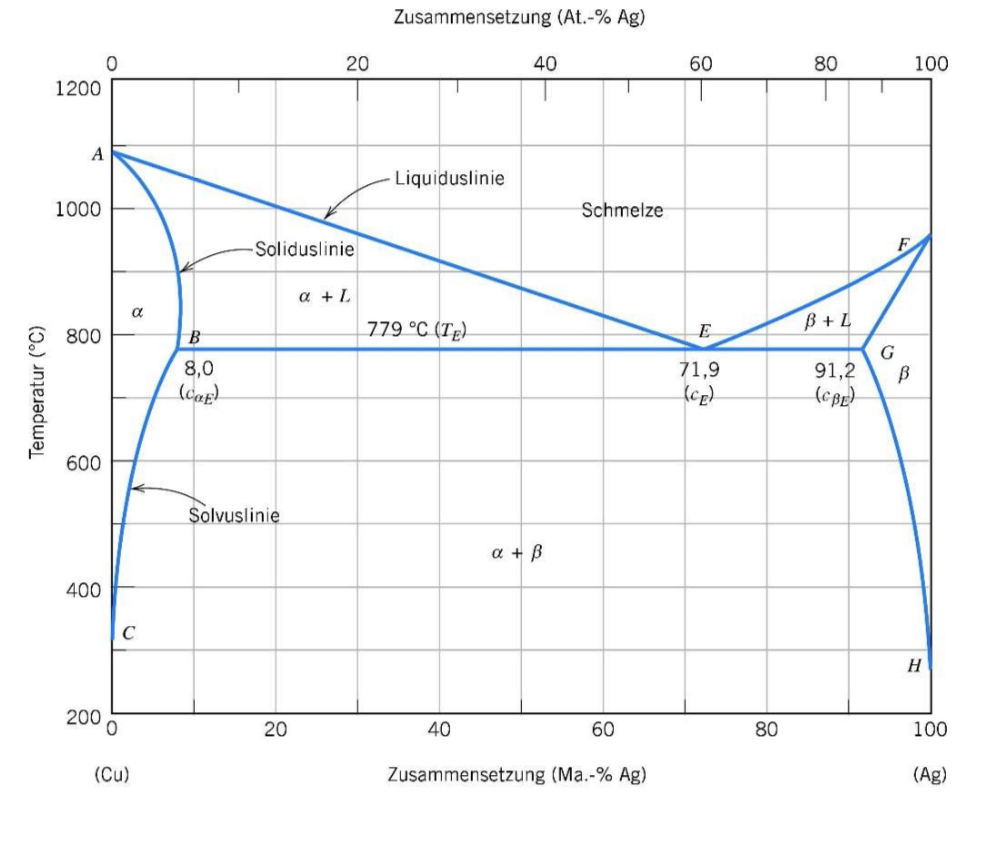
\includegraphics[width = 0.8\textwidth]{images/Materialwissenschaften/eutektisch_Phasendiagramm.jpeg}
    \caption{Phasendiagramm eines binären eutektischen Systems.}
    \label{fig:Phasendiagramm_eutektisch}
\end{figure}
\end{addmargin}

\noindent\textbf{12. Wie viele Parameter müssen in binären Systemen für Ein-, Zwei- und Dreiphasengebiete angegeben werden um deren Zustand zu bestimmen?}\\
\begin{addmargin}[25pt]{0pt}
Dieser Zusammenhang ist über die Gibbs'sche Phasenregel definiert:
\begin{equation}\label{eq:Gibbs_Phasenregel}
    P + F = K + N
\end{equation}
Dabei ist $P$ die Anzahl der vorliegenden Phasen, $F$ die Anzahl der Freiheitsgrade des Systems, $K$ die Anzahl der Komponenten im System und $N$ die Anzahl der Zustandvariablen. In einem binären System wie einer Kupfer-Silber Legierung ist $K = 2$. Da in unserem Fall der Druck immer als Standarddruck vorgegeben wird, ist die Temperatur die einzige Zustandsvariable, also $N = 1$. Damit ergibt sich für ein Einphasengebiet: $F = 2$ also sind Temperatur und Zusammensetzung unabhängig voneinander. Im Zweiphasengebiet ist $F = 1$ also ist für eine feste Temperatur die Zusammensetzung der festen und der flüssigen Phase vorgegeben, das habe wir bereits in Frage 6 dieses Kapitels gesehen. Im Dreiphasengebiet müssen sowohl Temperatur als auch Zusammensetzung einen bestimmten Wert haben, demnach st $F = 0$.\\ 
\end{addmargin}

\noindent\textbf{13. Welche Strukturen nimmt reines Eisen als Funktion der Temperatur an? Welche Eigenschaften haben diese? Wie gut ist jeweils die Löslichkeit von Kohlenstoff?}\\
\begin{addmargin}[25pt]{0pt}
Bei Raumtemperatur liegt Eisen als Ferrit oder $\alpha$-Eisen vor, dieses hat eine bcc-Struktur und Kohlenstoff ist darin nur schlecht löslich da in der bcc-Struktur nur wenig Zwischengitterplätze vorhanden sind auf denen sich Kohlenstoff einlagern könnte. Ferrit ist relativ weich und bis $768^\circ $C ferromagnetisch. Ab einer Temperatur von $912^\circ$C wandelt sich Ferrit allotrop in Austenit oder $\gamma$-Eisen um, dieses besitzt eine fcc-Struktur wodurch sich Kohlenstoff sehr gut in ihm lösen lässt. Austenit ist nicht ferromagnetisch. Im Temperaturbereich $1394^\circ$C bis $1538^\circ$C hat Eisen wieder eine bcc-Struktur und ähnliche Eigenschaften zu Ferrit, daher nennt man diese Form von Eisen auch $\delta$-Ferrit. Bei noch höheren Temperaturen schmilzt reines Eisen.\\
\end{addmargin}

\noindent\textbf{14. Was ist Zementit und welche Eigenschaften hat er?}\\
\begin{addmargin}[25pt]{0pt}
Zementit ist eine Eisen-Kohlenstoff-Verbindung mit der Formel \ce{Fe3C}. Es bildet sich wenn mehr Kohlenstoff vorhanden ist als in Eisen gelöst werden kann. Zementit ist sehr hart und spröde und eigentlich ein metastabiles Material, allerdings ist seine Lebenszeit extrem hoch.\\
\end{addmargin}

\noindent\textbf{15. Wodurch unterscheiden sich Stahl und Gusseisen?}\\
\begin{addmargin}[25pt]{0pt}
Stahl ist eine Legierung aus Eisen und Kohlenstoff bei der Kohlenstoff mit einem Massenanteil von $0,008-2,14 \%$ auftritt. Wohingegen Gusseisen einen deutlich höheren Kohlenstoffanteil mit $2,14-6,70 \%$ hat. Die Mikrostruktur von Stahl ist sehr charakteristisch, andererseits kann die Mikrostruktur von Gusseisen verschiedene Formen annehmen. In Gusseisen liegt der Kohlenstoff als Graphit vor und in Stahl ist er eingelagert, entweder in der $\alpha$-Phase oder in Zementit \ce{Fe3C} \\
\end{addmargin}


\subsection{Phasenumwandlungen}

\noindent\textbf{1. Welche Umwandlungsprozesse kennen Sie?}\\
\begin{addmargin}[25pt]{0pt}
Es gibt diffusionsabhängige Phasenübergänge bei denen die Anzahl oder die Zusammensetzung der Phasen unverändert bleibt, dann gibt es diffusionsabhängige Umwandlungen bei denen sich die Phasenzusammensetzung und häufig auch die Anzahl der Phasen ändert und schließlich gibt es noch Umwandlungen ohne Diffusionin eine metastabile Phase. Die Erstarrung eines reinen Metalls oder das Kornwachstum sind Beipsiele für Phasenübergänge bei denen die Anzahl oder die Zusammensetzung der Phasen unverändert bleibt. Die eutektoide Reaktion ist ein Beispiel für eine Änderung der Phasenzusammensetzung.\\
\end{addmargin}

\noindent\textbf{2. Welche beiden Prozesse sind für die Umwandlung nötig?}\\
\begin{addmargin}[25pt]{0pt}
Um die Phasenumwandlung beginnen zu können muss zunächst ein kleiner Keim der neuen Phase entstehen und danach muss dieser wachsen, diese Prozesse nennt man Keimbildung und Kristallwachstum. In der Keimbildung entstehen typischerweise zahlreiche kleine Partikel und nicht nur ein einziges. Beim Kristallwachstum wachsen dann nicht alle dieser kleinen Partikel sondern manche zerfallen auch wieder. \\
\end{addmargin}

\noindent\textbf{3. Welche Arten von Keimbildung werden unterschieden?}\\
\begin{addmargin}[25pt]{0pt}
Es existiert dei homogene Keimbildung, dabei entstehen die Keime gleichförmig im Volumen der Ausgangsphase und dann gibt es noch die heterogene Keimbildung bei der Keime sich bevorzugt an Inhomogenitäten wie Korngrenzen, Oberflächen, Verunreinigungen oder Versetzungen bilden. Die heterogene Keimbildung ist der Effekt, welcher in Phasenumwandlungen in der Natur die Ursache ist, da diese Keime sich energetisch günstiger bilden können.\\
\end{addmargin}

\noindent\textbf{4. Welche Anteile hat die freie Enthalpie eines Keims
und wie hängen diese von seinem Radius ab? }\\
\begin{addmargin}[25pt]{0pt}
Bei der Phasenumwandlung von flüssig in fest und der Annahme von homogener Keimbildung hat die freie Enthalpie 2 Anteile, einmal einen Oberflächenanteil und einen Volumenanteil. Der Volumenanteil berüclsichtigt die Differenz der freien Enthalpie in fester und flüssiger Phase pro Volumen, diese Größe ist $\Delta G_V$, multipliziert man diesen Wert mit dem Volumen $\frac{4}{3}\pi r^3$ des Keims erhält man die gesamte Enthalpieänderung aufgrund des Volumens. Der zweite Anteil betrachtet die freie Grenzflächenenthalpie pro Oberfläche des Keims, dieser Wert wird $\gamma$ genannt analog zum Volumen muss hier $\gamma$ einfach mit der Oberfläche $4\pi r^2$ multipliziert werden um die Enthalpieänderung zu bestimmen. Die gesamte Enthalpieänderung durch einen kugelförmigen Keim von Radius $r$ ist:
\begin{equation}\label{eq:enthalpie_homogene_Keimbildung}
    \Delta G = \frac{4}{3}\pi r^3 \Delta G_V + 4\pi r^2 \gamma
\end{equation}
Für die Umwandlung flüssig $\rightarrow$ fest ist allgemein: $\Delta G_V <0$ und $\gamma >0$\\
\end{addmargin}

\noindent\textbf{5. Wie hängt die Gesamtenergie des Keims von seinem Radius ab?}\\
\begin{addmargin}[25pt]{0pt}
In Abbildung \ref{fig:Enthalpie_Phasenumwandlung} sind der Oberflächenanteil (rot), der Volumenanteil (blau) und die Gesamtenthalpieänderung (grün) gegen den Radius geplottet. Man erkennt, dass ab einem kritischen Radius $r^*$ die Keime stabil sind und weiter wachsen, bei niedrigeren Radien lösen sie sich wieder auf. Aus der Bedingung $\frac{\si{d} \Delta G}{\si{d}r} = 0$ am Ort des kritischen Radius findet man:
\begin{align}\label{eq:kritischer_Radius}
    r^* &=-\frac{2\gamma}{\Delta G_V}\\\label{eq:Aktivierungsenergie}
    \Delta G^* &= \frac{16\pi\gamma^3}{3(\Delta G_V)^2}
\end{align}
\begin{figure}[h]
    \centering
    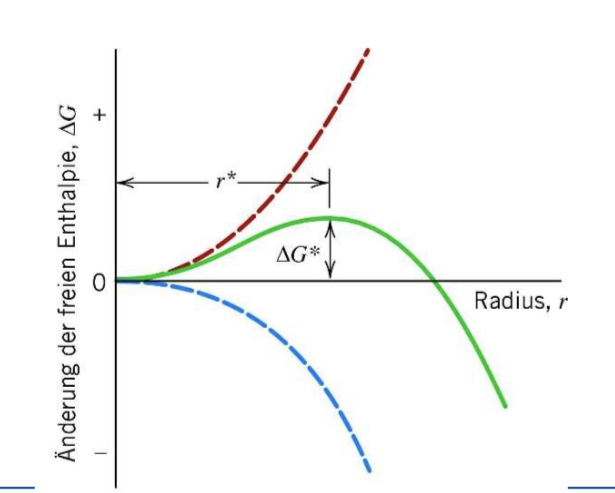
\includegraphics[width = 0.8\textwidth]{images/Materialwissenschaften/Enthalpie_Phasneumwandlung.jpeg}
    \caption{In rot ist der Oberflächenanteil, in blau der Volumenanteil und in grün die gesamte Änderung der Enthalpieänderung eines Keims zu sehen, der kritische Radius $r^*$ und die Aktivierungsenergie $\Delta G^*$ sind ein Maß dafür ab welchen Bedingungen die Keime weiter wachsen und sich nicth wieder auflösen}
    \label{fig:Enthalpie_Phasenumwandlung}
\end{figure}
\end{addmargin}

\noindent\textbf{6. Wie hängen der kritische Radius $r^*$, die Aktivierungsenergie $\Delta G^*$ 
und die Anzahl der stabilen Keime $n^*$ von der Temperatur ab?
}\\
\begin{addmargin}[25pt]{0pt}
In den Gleichungen \ref{eq:kritischer_Radius} und \ref{eq:Aktivierungsenergie} ist $\Delta G_V$ temperaturabhängig und $\gamma$ nicht. Für die Temperaturabhängigkeit von $\Delta G_V$ nutzt man folgenden Zusammenhang:
\begin{equation}\label{eq:Umwandlungswärme}
    \Delta G_V = \frac{\Delta H_f \cdot (T_S - T)}{T_S}
\end{equation}
dabei ist $T_S$ die Schmelztemperatur und $\Delta H_f$ die bei Erstarrung freigesetzte Wärmemenge. Eingesetzt in die Gleichungen  \ref{eq:kritischer_Radius} und \ref{eq:Aktivierungsenergie} ergibt das:
\begin{align}
    r^* &= \left( - \frac{2\gamma T_S}{\Delta H_f}\right) \frac{1}{T_S - T}\\
    \Delta G^* &= \left( \frac{16\pi \gamma^3 T_S^2}{3(\Delta H_f)^2}\right) \frac{1}{(T_S - T)^2} 
\end{align}
Die Anzahl der stabilen Keime (für diese gilt: $r>r^*$) ist gegeben mit:
\begin{equation}
    n^* = K_1 \exp(-\frac{\Delta G^*}{k_BT})
\end{equation}
\end{addmargin}

\noindent\textbf{7. Welcher weitere Prozess ist für die Keimbildungsrate wichtig und was bewirkt dies für ihre Temperaturabhängigkeit?}\\
\begin{addmargin}[25pt]{0pt}
Die Keimbildungsrate hängt sowohl von der Anzahl der stabilen Keime als auch von der Anlagerungsrate an diese Keime ab. Die Anzahl der stabilen Keime steigt bei Temperaturen unterhalb $T_S$ an, wohingegen die Anlagerungsrate abnimmt. Dadurch ergibt sich ein Maximum der Keimbildungsrate bei einer bestimmten Temperatur unterhalb der Schmelztemperatur. Dieses Maximum wird als Unterkühlung bezeichnet.\\
\end{addmargin}

\noindent\textbf{8. Warum ist die Keimbildung an Ober- bzw. Grenzflächen leichter möglich als im Volumen und welche Konsequenzen hat dies?}\\
\begin{addmargin}[25pt]{0pt}
Die freie Grenzflächenenthalpie $\gamma$ ist an Oberflächen deutlich geringer als im Volumen wodurch sich Keime bevorzugt an Ober-/Grenzflächen bilden. Daraus folgt dass die heterogene Keimbildung energetisch deutlich wahrscheinlicher auftritt als die homogene Keimbildung.\\
\end{addmargin}

\noindent\textbf{9. Wie hängt die Mikrostruktur von der Umwandlungstemperatur ab?}\\
\begin{addmargin}[25pt]{0pt}
Bei Temperaturen nahe $T_S$ ist die Keimbildungsrate gering aber die Wachstumsrate hoch, dadurch entstehen wenige Körner die dafür größer sind. Bei Temperaturen weit unterhalb der Schmelztemperaturen tritt genau der entgegengesetzte Effekt ein, es entstehen viele kleine Körner.\\
\end{addmargin}

\noindent\textbf{10. Wie hängt bei Umwandlungen im festen Zustand
der Umwandlungsgrad von der Umwandlungstemperatur ab?}\\
\begin{addmargin}[25pt]{0pt}
\begin{figure}[h]
    \centering
    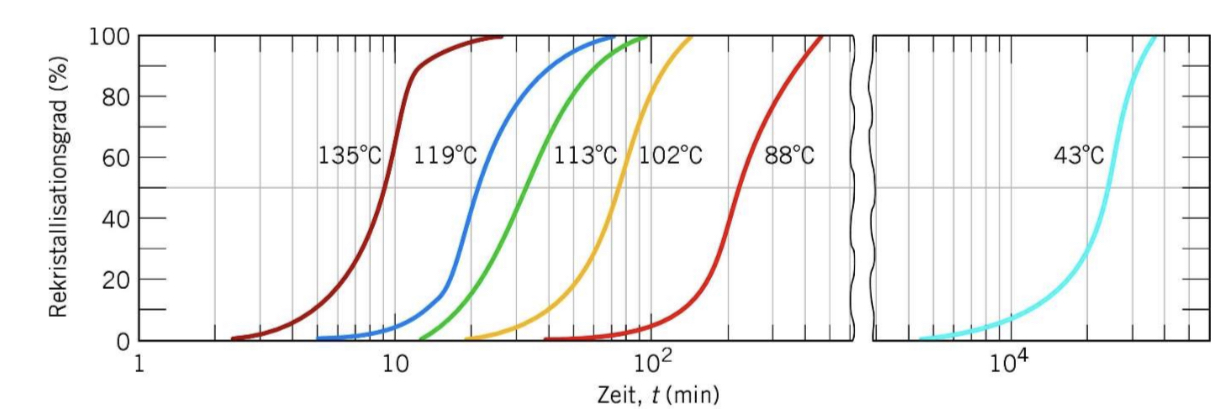
\includegraphics[width = 0.8\textwidth]{images/Materialwissenschaften/Umwandlungsgrad.jpeg}
    \caption{Der Umwandlungsgrad in Abhängigkeit von der Zeit und der Temperatur}
    \label{fig:Umwandlungsgrad}
\end{figure}
In Abbildung \ref{fig:Umwandlungsgrad} ist der Umwandlungsgrad in Abhängigkeit von der Zeit und der Temperatur dargestellt. Man erkennt, dass die Kurven immer S-förmig sind und bei geringeren Temperaturen länger benötigen um Keime zu bilden und die Umwandlung zu starten. \\
\end{addmargin}

\noindent\textbf{11. Was ist in einem Zeit-Temperatur-Umwandlungsdiagramm aufgetragen?}\\
\begin{addmargin}[25pt]{0pt}
\begin{figure}[h]
    \centering
    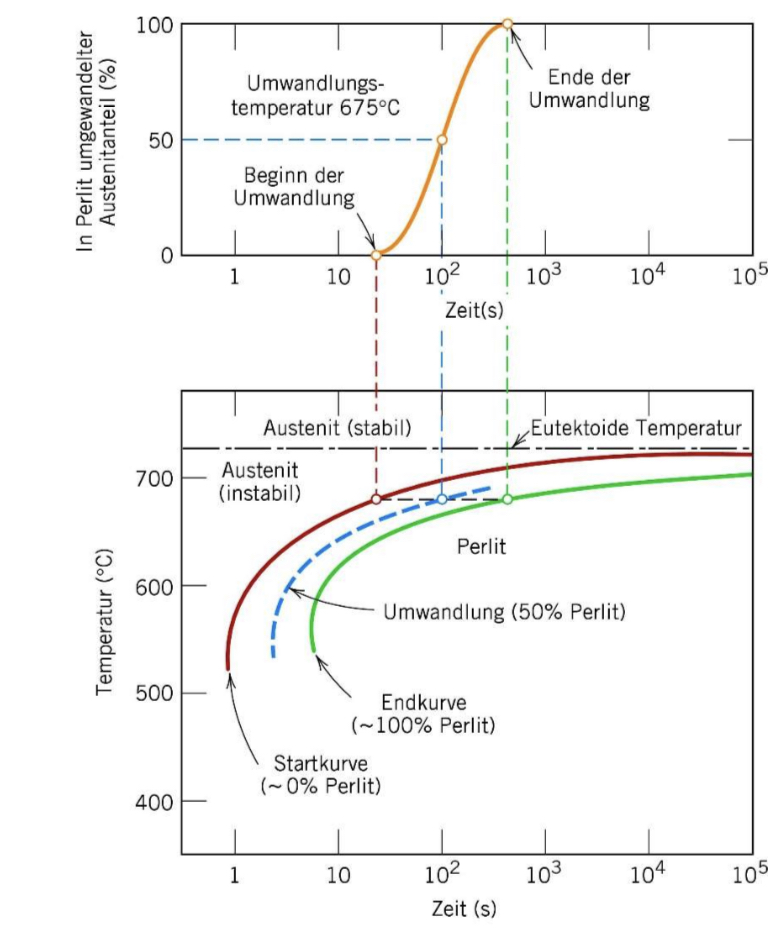
\includegraphics[width = 0.8\textwidth]{images/Materialwissenschaften/TTT_diagram.jpeg}
    \caption{Zeit-Temperatur-Umwandlungsdiagramm dargestellt auf 2 Varianten}
    \label{fig:TTT_diagram}
\end{figure}
In Abbildung \ref{fig:TTT_diagram} sind die beiden Varianten eines Zeit-Temperatur-Umwandlungsdiagrammes zu sehen. 
\end{addmargin}

\subsection{Keramiken und Gläser}
\noindent\textbf{1. Aus was bestehen Keramiken und von welcher Art sind die Bindungen?}\\
\begin{addmargin}[25pt]{0pt}
Keramiken sind anorganische Verbindungen aus Metallen und Nichtmetallen. Die Bindungen sind entweder ionischer oder kovalenter Natur, abhängig von den Elektronegativitäten der beteiligten Elemente. Die charateristischen keramischen Eigenschaften werden erst durch Hochtemperaturbehandlung erzielt. \\
\end{addmargin}

\noindent\textbf{2. Wodurch sind die Kristallstrukturen bestimmt?}\\
\begin{addmargin}[25pt]{0pt}
Bei einem ionischen Bindungscharakter sind die Beträge der elektrischen Ladungen und das Größenverhältnis von Kation zu Anion relevant für die Kristallstruktur. Stabile Kristalstrukturen zeichnen sich dabei dadurch aus, dass die als feste Kugeln angenommenen Ionen in Kontakt zueinander stehen und dabei immer Kation und Anion sich berühren. Damit ergeben sich in Abhängigkeit des Radienverhältnisses $\frac{r_K}{r_A}$ verschiedene mögliche Kristallstrukturen:
\begin{align*}
    \frac{r_K}{r_A} &= 0,225-0,414 \rightarrow \text{Koordinationszahl 4, Tetraeder}\\
    \frac{r_K}{r_A} &= 0,414-0,732 \rightarrow \text{Koordinationszahl 6, Oktaeder}\\
    \frac{r_K}{r_A} &= 0,732-1     \hspace{0.75cm}\rightarrow \text{Koordinationszahl 8, Würfel}
\end{align*}\\
\end{addmargin}

\noindent\textbf{3. Wie bilden sich dichteste Kugelpackungen in Keramiken aus?}\\
\begin{addmargin}[25pt]{0pt}
Es entstehen dicht gepackte Schichten aus großen Anionen und kleineren Kationen in den Zwischenräumen. 2 benachbarte schichten von Anionen können dabei entweder eine Tetraederposition bilden, dabei werden 3 Anionen aus einer mit einem Anion aus der zweiten Schicht verwendet, oder es bildet sich eine Oktaederposition mit jeweils 3 Ionen aus jeder Schicht. In den Zwischenräumen lagern sich jeweils Kationen ein.  \\
\end{addmargin}

\noindent\textbf{4. Welche Silikatkeramiken kennen sie und wie sind deren Strukturen?}\\
\begin{addmargin}[25pt]{0pt}
Silikatmaterialien bestehen aus \ce{(SiO4)^4-}-Tetraedern. Die Klassifizierung erfolgt dann nach der Anordnung dieser Tetraeder. Siliziumdioxid hat die Eigenschaft, dass benachbarte Tetraeder 2 O-Atome an ihren Ecken sich teilen, dadurch ist das gesamte 3-dimensionale Netzwerk elektrisch neutral. Siliziumdioxid hat eine sehr starke Bindung wodurch es eine hohe Schmelztemperatur besitzt. Silikatische Gläser sind in Abbildung \ref{fig:Silikatgläser} dargestellt. Auf der linken Seite sieht man ein reines Silikatglas und rechts Fensterglas, das sind Silikatgläser denen andere Materialien wie \ce{CaO} oder \ce{Na2O} zugegeben wurden.
\begin{figure}[h]
    \centering
    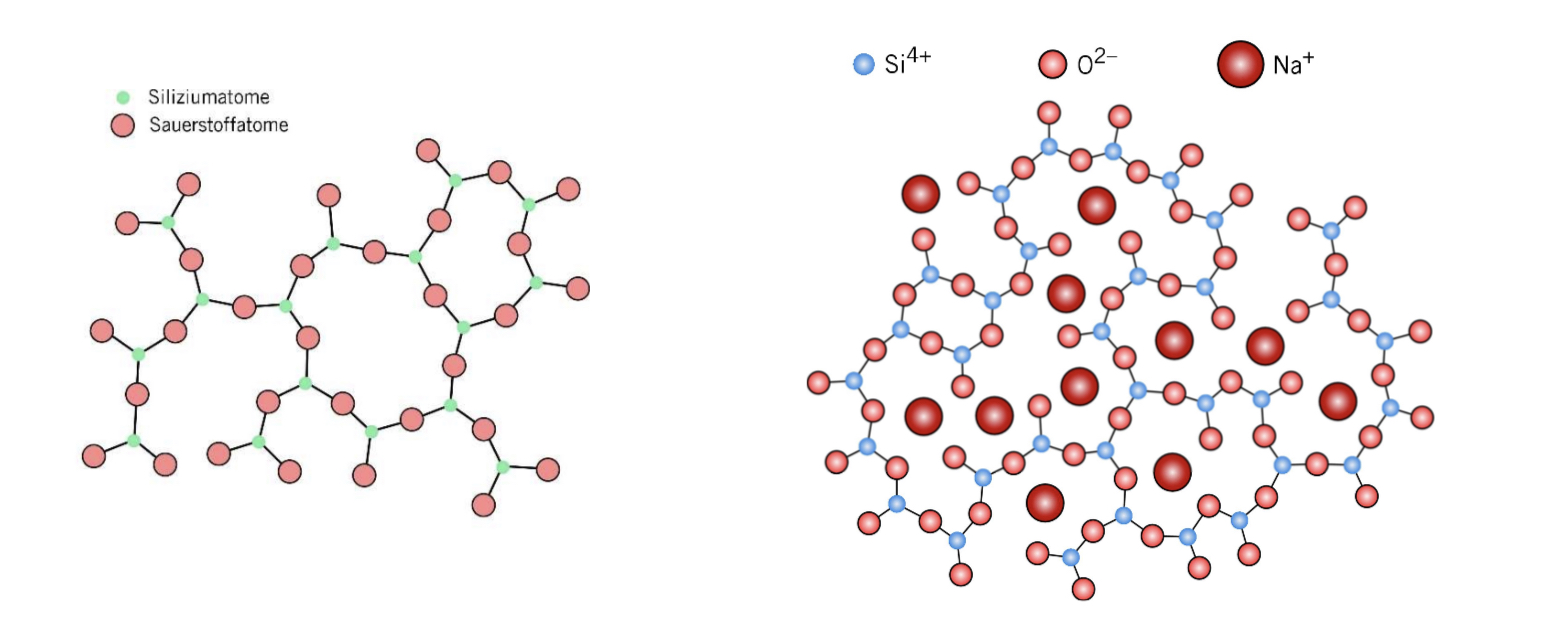
\includegraphics[width = 0.8\textwidth]{images/Materialwissenschaften/Silikatische_glaser.jpeg}
    \caption{Silikatgläser, rein auf der linken Seite und mit Zusatz rechts}
    \label{fig:Silikatgläser}
\end{figure}
Schichtsilikate sind die letzte Form der Silikatmaterialien, bei ihnen liegt eine zweidimensionale Schichtstruktur vor, bei der drei oder vier O-Atome an Tetraederecken gemeinsam genutzt werden, es entstehen \ce{(Si2O5)^2-} Verbindungen. Ein bekanntes Beispiel für ein Schichtsilikat ist der Ton.\\
\end{addmargin}

\noindent\textbf{5. Welche allotropen Formen nimmt Kohlenstoff an?}\\
\begin{addmargin}[25pt]{0pt}
Kohlenstoff kann entweder als Fullerene \ce{C60} vorliegen oder als Kohlenstoff-Nanoröhrchen. Fullerene sind hohle Kugeln, welche aus 60 C-Atomen bestehen die in 5- und 6-Ringen angeordnet sind. Im Festkörper bilden mehrere Fullerene eine bcc-Struktur und wirken als Isolator. Kohlenstoff-Nanoröhrchen sind Graphitschichten, welche zu einer zylindrigen Form aufgerollt wurden. Diese Zylinder werden mit \ce{C60}-Halbkugeln abgedeckt. Kohlenstoff-Nanoröhrchen haben einen Durchmesser von unter 100 nm  und einer Länge die die größer ist als 1000 mal der Durchmesser.\\
\end{addmargin}

\noindent\textbf{6. Welche Punktdefekte sind in Keramiken hauptsächlich vorhanden?}\\
\begin{addmargin}[25pt]{0pt}
In Keramiken mit einer regelmäßigen Anordnung von Kationen und Anionen kann entweder ein Kation oder ein Anion fehlen oder es können auch 2 Kationen den gleichen Zwischengitterplatz einnehmen, siehe Abbildung \ref{fig:Fehlstellen_Keramiken}. Ein Anion auf einem Zwischengitterplatz ist sehr unwahrscheinlich da Anionen sehr viel größer sind als Kationen. Diese beschriebenen Gitterdefekte können jedoch nicht einzeln auftreten, da in Keramiken die Elektroneutralität eingehalten werden muss. Deswegen gibt es in der Realität immer entweder einen Schottky-Defekt, also eine Kombination aus Anion- und Kationfehlstelle oder einen Frenkel-Defekt, das ist eine Kombination aus Kationfehlstelle und einem zusätzlichen Zwischengitterkation.\\
\begin{figure}[h]
    \centering
    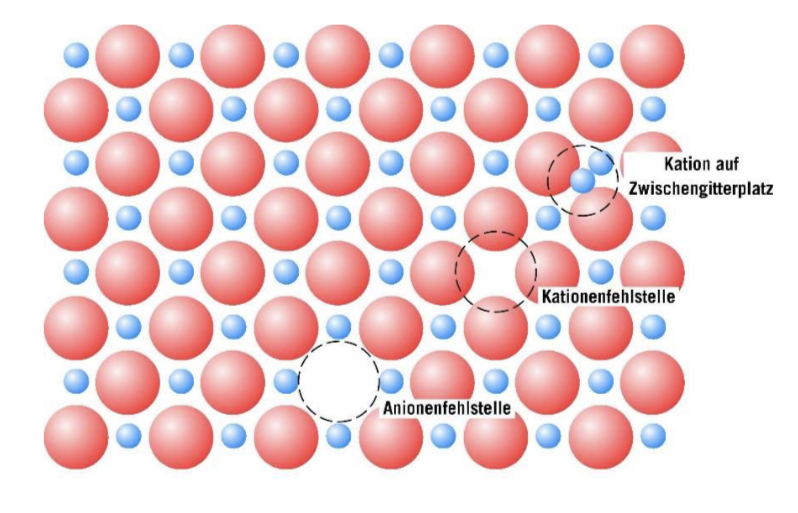
\includegraphics[width = 0.8\textwidth]{images/Materialwissenschaften/Fehlstellen_Keramiken.jpeg}
    \caption{Die verschiedenen Arten von Fehlstellen in Keramiken}
    \label{fig:Fehlstellen_Keramiken}
\end{figure}
\end{addmargin}

\noindent\textbf{7. Wie sehen Phasendiagramme von Keramiken aus?}\\
\begin{addmargin}[25pt]{0pt}
Phasendiagramme von einem zweikomponentigen System, wie zum Beispiel \ce{Al2O3}-\ce{Cr2O3}, sind wie bei einem Metall-Metall-System. Es existiert ebenso ein Mischkraitall, eine flüssige Phase und ein Zwei-Phasengebiet mit Solidus- und Liquiduslinie.\\
\end{addmargin}

\noindent\textbf{8. Warum sind Keramiken so zerbrechlich?}\\
\begin{addmargin}[25pt]{0pt}
Keramiken sind sehr zerbrechlich und spröde, außerdem weisen sie deutlich geringere Bruchfestigkeiten auf als von den atomaren Bindungskräften vorhergesagt. Dafür gibt es 2 Gründe:\\
\begin{enumerate}
    \item mikroskopische/nanoskopische Defekte, wie Korngrenzen, Poren, Einschlüsse oder Mikrorisse wirken spannungsverstärkend
    \item in Keramiken gibt es keinen Mechanismus, welcher Risse abbremst oder teilt 
\end{enumerate}
\end{addmargin}

\noindent\textbf{9. Was ist Glaskeramik und wie wird sie hergestellt?}\\
\begin{addmargin}[25pt]{0pt}
Glaskeramik besteht aus Kristalliten, welche in eine glasförmige Matrix eingebettet sind. Glaskeramiken bestehen hauptsächlich aus \ce{SiO2}, außerdem sind \ce{Na2O}, \ce{Al2O3}, \ce{B2O3}, \ce{TiO2} und \ce{As2O3} in ihr enthalten. Die Kristallite und das Glas haben einen ähnlichen Brechungsindex wodurch die Glaskeramik durchsichtig wird. Glaskeramiken haben einen niedrigen Wärmeausdehnungskoeffizienten, daher sind sie ideal zum Bau von Kochfeldern oder Haltern in Hochtemperatur-Brennstoffzellen. Zur Herstellung von Glaskeramiken werden zuerst die Bestandteile geschmolzen, danach bei einer etwas niedrigeren Temperatur geformt, als nächstes wird die Schmelze abgekühlt und danach bei verschiedenen Temperaturen gehalten damit erst Keime sich bilden können und diese danach wachsen. Schließlich ist die Glaskeramik in der gewünschten Form erstarrt. \\
\end{addmargin}


\noindent\textbf{10. Wie wird die Glastemperatur bestimmt?}\\
\begin{addmargin}[25pt]{0pt}
Bei der Herstellung von Gläsern wird die Schmelze gekühlt, ab der Schmelztemperatur beginnt dann die Kristallisation und es entsteht ein kristalliner Feststoff, dessen spezifisches Volumen deutlich geringer ist als man es für Glas erwartet, tritt dieser Fall ein hat die Glaserstellung nicht funktioniert, weil zur Glasherstellung keine Kristallisation auftreten soll. Schafft man es die Kristallisation bei der Schmelztemperatur zu unterdrücken, so wird man ab der Glasübergangstemperatur einen fließenden Übergang von Schmelze zu Glas beobachten. Trägt man das Spezifische Volumen gegen die Temperatur auf so wird bei der erfolgreichen Herstellung von Glas an der Glasübergangstemperatur eine stetige aber nicht differenzierbare Stelle zu sehen sein. Stellt man jedoch einen kristallinen Feststoff her so erkennt man bei der Schmelztemperatur und Unstetigkeit. \\
\end{addmargin}

\noindent\textbf{11. Wie verhält sich die Viskosität von Gläsern mit der Temperatur?}\\
\begin{addmargin}[25pt]{0pt}
In Abbildung \ref{fig:glas_viskosität} kann man die Viskosität einiger Gläser gegen die Temperatur aufgetragen sehen.
\begin{figure}[h]
    \centering
    \includegraphics[width = 0.8\textwidth]{images/Materialwissenschaften/glas_viskosität.jpeg}
    \caption{Viskosität einiger Gläser gegen die Temperatur aufgetragen}
    \label{fig:glas_viskosität}
\end{figure}
\end{addmargin}




\subsection{Komposite}
\noindent\textbf{1. Welche Vorteile bieten Kompositmaterialien?}\\
\begin{addmargin}[25pt]{0pt}
Durch die geschickte Kombination von mehreren Werkstoffen in ein Verbundwerkstoff können gezielt wünschenswerte Eigenschaften erzielt werden. Damit kann man zum Beispiel ein Material erschaffen, welches eine hohe Festigkeit aber gleichzeitig eine geringe Dichte aufweist. Kompositmaterialien bestehen dabei häufig aus einer duktilen Matrix in die feste Partikel eingelagert sind.\\
\end{addmargin}

\noindent\textbf{2. Welche Rolle spielen die duktile Matrix und die festen Partikel für die mechanischen Eigenschaften?}\\
\begin{addmargin}[25pt]{0pt}
Die duktile Matrix sorgt dafür dass die Partikel räumlich voneinander getrennt sind aber gleichzeitig an festen Orten zusammengehalten werden. Weiterhin überträgt die MAtrix die extern angelegte mechanische Spannung. Außerdem schützt die Matrix die Partikel vor diversen Arten der Beschädigung. Die Partikel hingegen sorgen für einen hohen E-Modul des gesamten Materials und erhöhen die spezifische Festigkeit.\\
\end{addmargin}

\noindent\textbf{3. Warum müssen die Fasern eine gewisse Mindestlänge haben?}\\
\begin{addmargin}[25pt]{0pt}
An den Enden der Phase liegt keine Spannung an, die Spannung steigt linear bis zur Mitte der Faser. Falls die Faser zu kurz ist, liegt kann die Faser in der Mitte nur eine Spannung aufnehmen, welche kleiner ist als die anliegende Spannung. Ab der Mindestlänge der Faser kann die Faser die anliegende Spanung kompensieren. Ist die Faser noch länger so verbreitert sich der Bereich in dem die anliegende Spannung kompensiert werden kann und die Faser wird noch stabiler.\\
\end{addmargin}

\noindent\textbf{4. Wie sieht die Spannungs-Dehnungs-Kurve eines Komposits mit ausgerichteten Fasern aus und was passiert in den verschiedenen Stadien?}\\
\begin{addmargin}[25pt]{0pt}
In Abbildung \ref{fig:Faser_Spannung_Dehnung} kann man die Spannungs-Dehnungs-Kurve von den einzelnen Fasern, der einzelnen Matrix und des Verbundwerkstoffes sehen. Zunächst verformen sich beide Komponenten elastisch, danach kommt es zu plastischer Deformation der Matrix und schließlich reißen die Fasern, allerdings hat der Verbundwerkstoff den Vorteil, dass Risse der Fasern nicht katastrophal sind da die plastisch verformte Matrix immer noch Stabilität bietet.  \\ 
\begin{figure}[h]
    \centering
    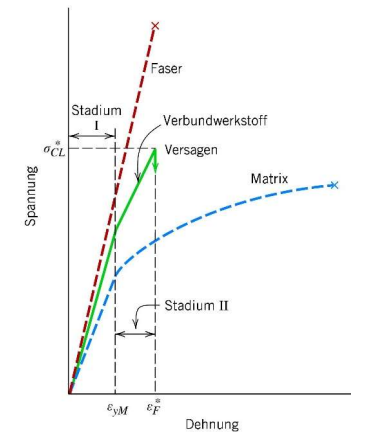
\includegraphics[width = 0.65\textwidth]{images/Materialwissenschaften/Faser_spannung-Dehnung.png}
    \caption{Spannungs-Dehnungs-Diagramm von Faser, Matrix und Verbundwerkstoff}
    \label{fig:Faser_Spannung_Dehnung}
\end{figure}
\end{addmargin}

\noindent\textbf{5. Durch welche mechanischen Eigenschaften zeichnen sich Kohlefasern aus?}\\
\begin{addmargin}[25pt]{0pt}
Kohlefasern haben einen sehr hohen E-Modul, eine hohe spezifische Festigkeit und sind chemisch sehr widerstandsfähig. Kohlefasern bestehen aus Graphit und aus nichtkristallinen Bereichen. \\
\end{addmargin}

\noindent\textbf{6. Welche Vorteile bieten Kohlenstoff-Nanoröhrchen gegen Kohlefasern und was bedeutet dies für die Eigenschaften der Komposite?}\\
\begin{addmargin}[25pt]{0pt}
Kohlenstoff-Nanoröhrchen können als deutlich kleinere Partikel in die Matrix eingelagert werden (Nanometer anstatt Mikrometer) wodurch der Kontakt zur Matrix an der Grenzfläche deutlich verbessert wird. Daraus resultieren verbesserte mechanische, thermische und elektrische Eigenschaften. Diese Komposite können sowohl leitend als auch halbleitend sein. Komposite mit Kohlenstoff-Nanoröhrchen haben außerdem eine hohe Wärmeleitfähigkeit und sehr niedrige Massendichte.  \\
\end{addmargin}

\noindent\textbf{7. Welche Schwierigkeiten gibt es bei der Präparation von Nanokompositen aus einer Polymermatrix und Kohlenstoff-Nanoröhrchen?}\\
\begin{addmargin}[25pt]{0pt}
Kohlenstoff-Nanoröhrchen haben untereinander eine starke Anziehung aufgrund der van-der-Waals-Wechselwirkung, dadurch bilden sich bevorzugt Cluster welche in Nanokompositen nicht gewünscht sind. Obwohl CNTs zur Matrix eine große Kontaktfläche haben, wodurch sich eine gute Leitfähigkeit ergibt, so sind sie dennoch schlecht an sie angebunden, dadurch werden sie bei Belastung eventuell mechanisch herausgezogen. Diese Schwierigkeit versucht man zu lösen indem man die Grenzfläche mit chemischen Reaktionen an die Anwendung anpasst.  \\
\end{addmargin}

\noindent\textbf{8. Welche Art von Struktur wird von vielen biologischen Kompositen gebildet, welche Vorteile bietet dies und welche Mechanismen liegen zugrunde?}\\
\begin{addmargin}[25pt]{0pt}
Biologische Materialien sind häufig in einer hierarchischen Struktur aufgebaut, siehe Abbildung \ref{fig:hierarchie}. Die hierarchische Struktur sorgt dafür, dass sich Risse schlechter ausbreiten können und sich die Spannung gut verteilt und so kein Bereich zu stark belastet wird. In der hierarchischen Struktur gilt: je mehr hierarchische Levels vorhanden sind umso höher ist die Steifigkeit und die Zähigkeit des Kompositmaterials \\
\begin{figure}[h]
    \centering
    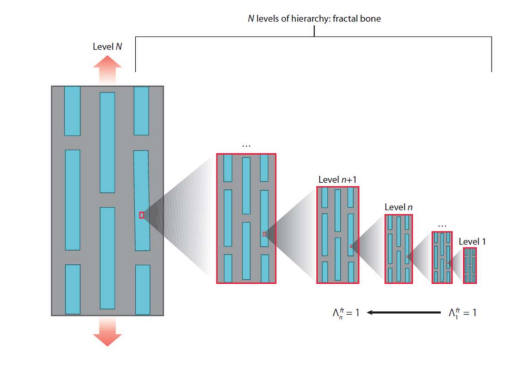
\includegraphics[scale = 0.85]{images/Materialwissenschaften/hierarchische_struktur.png}
    \caption{Hierarchische Struktur in biologischen Materialien}
    \label{fig:hierarchie}
\end{figure}
\end{addmargin}

